\documentclass[]{book}
\usepackage{lmodern}
\usepackage{amssymb,amsmath}
\usepackage{ifxetex,ifluatex}
\usepackage{fixltx2e} % provides \textsubscript
\ifnum 0\ifxetex 1\fi\ifluatex 1\fi=0 % if pdftex
  \usepackage[T1]{fontenc}
  \usepackage[utf8]{inputenc}
\else % if luatex or xelatex
  \ifxetex
    \usepackage{mathspec}
  \else
    \usepackage{fontspec}
  \fi
  \defaultfontfeatures{Ligatures=TeX,Scale=MatchLowercase}
\fi
% use upquote if available, for straight quotes in verbatim environments
\IfFileExists{upquote.sty}{\usepackage{upquote}}{}
% use microtype if available
\IfFileExists{microtype.sty}{%
\usepackage{microtype}
\UseMicrotypeSet[protrusion]{basicmath} % disable protrusion for tt fonts
}{}
\usepackage[margin=1in]{geometry}
\usepackage{hyperref}
\hypersetup{unicode=true,
            pdftitle={Animal Environmental Science},
            pdfauthor={Sangrak Lee; Youngjun Na},
            pdfborder={0 0 0},
            breaklinks=true}
\urlstyle{same}  % don't use monospace font for urls
\usepackage{natbib}
\bibliographystyle{apalike}
\usepackage{longtable,booktabs}
\usepackage{graphicx,grffile}
\makeatletter
\def\maxwidth{\ifdim\Gin@nat@width>\linewidth\linewidth\else\Gin@nat@width\fi}
\def\maxheight{\ifdim\Gin@nat@height>\textheight\textheight\else\Gin@nat@height\fi}
\makeatother
% Scale images if necessary, so that they will not overflow the page
% margins by default, and it is still possible to overwrite the defaults
% using explicit options in \includegraphics[width, height, ...]{}
\setkeys{Gin}{width=\maxwidth,height=\maxheight,keepaspectratio}
\IfFileExists{parskip.sty}{%
\usepackage{parskip}
}{% else
\setlength{\parindent}{0pt}
\setlength{\parskip}{6pt plus 2pt minus 1pt}
}
\setlength{\emergencystretch}{3em}  % prevent overfull lines
\providecommand{\tightlist}{%
  \setlength{\itemsep}{0pt}\setlength{\parskip}{0pt}}
\setcounter{secnumdepth}{5}
% Redefines (sub)paragraphs to behave more like sections
\ifx\paragraph\undefined\else
\let\oldparagraph\paragraph
\renewcommand{\paragraph}[1]{\oldparagraph{#1}\mbox{}}
\fi
\ifx\subparagraph\undefined\else
\let\oldsubparagraph\subparagraph
\renewcommand{\subparagraph}[1]{\oldsubparagraph{#1}\mbox{}}
\fi

%%% Use protect on footnotes to avoid problems with footnotes in titles
\let\rmarkdownfootnote\footnote%
\def\footnote{\protect\rmarkdownfootnote}

%%% Change title format to be more compact
\usepackage{titling}

% Create subtitle command for use in maketitle
\newcommand{\subtitle}[1]{
  \posttitle{
    \begin{center}\large#1\end{center}
    }
}

\setlength{\droptitle}{-2em}

  \title{Animal Environmental Science}
    \pretitle{\vspace{\droptitle}\centering\huge}
  \posttitle{\par}
    \author{Sangrak Lee; Youngjun Na}
    \preauthor{\centering\large\emph}
  \postauthor{\par}
      \predate{\centering\large\emph}
  \postdate{\par}
    \date{Last update: 2019-04-01}

\usepackage{booktabs}

\begin{document}
\maketitle

{
\setcounter{tocdepth}{1}
\tableofcontents
}
\chapter*{Welcome}\label{welcome}
\addcontentsline{toc}{chapter}{Welcome}

This is the website for \textbf{``Animal environmental science''}. To
understanding individual animals, we have to understand the relationship
they have with their environment. This book will focus at the
interaction between animals and the environment.

This website is (and will always be) \textbf{free to use}, and is
licensed under the
\href{http://creativecommons.org/licenses/by-nc-nd/3.0/us/}{Creative
Commons Attribution-NonCommercial-NoDerivs 3.0} License. The book is
written in \href{https://rmarkdown.rstudio.com}{RMarkdown} with
\href{https://bookdown.org}{bookdown}. Some photographs used in this
book was from \href{https://unsplash.com/}{Unsplash.com}. If you click
the download button up above, you can download the PDF version of the
book.

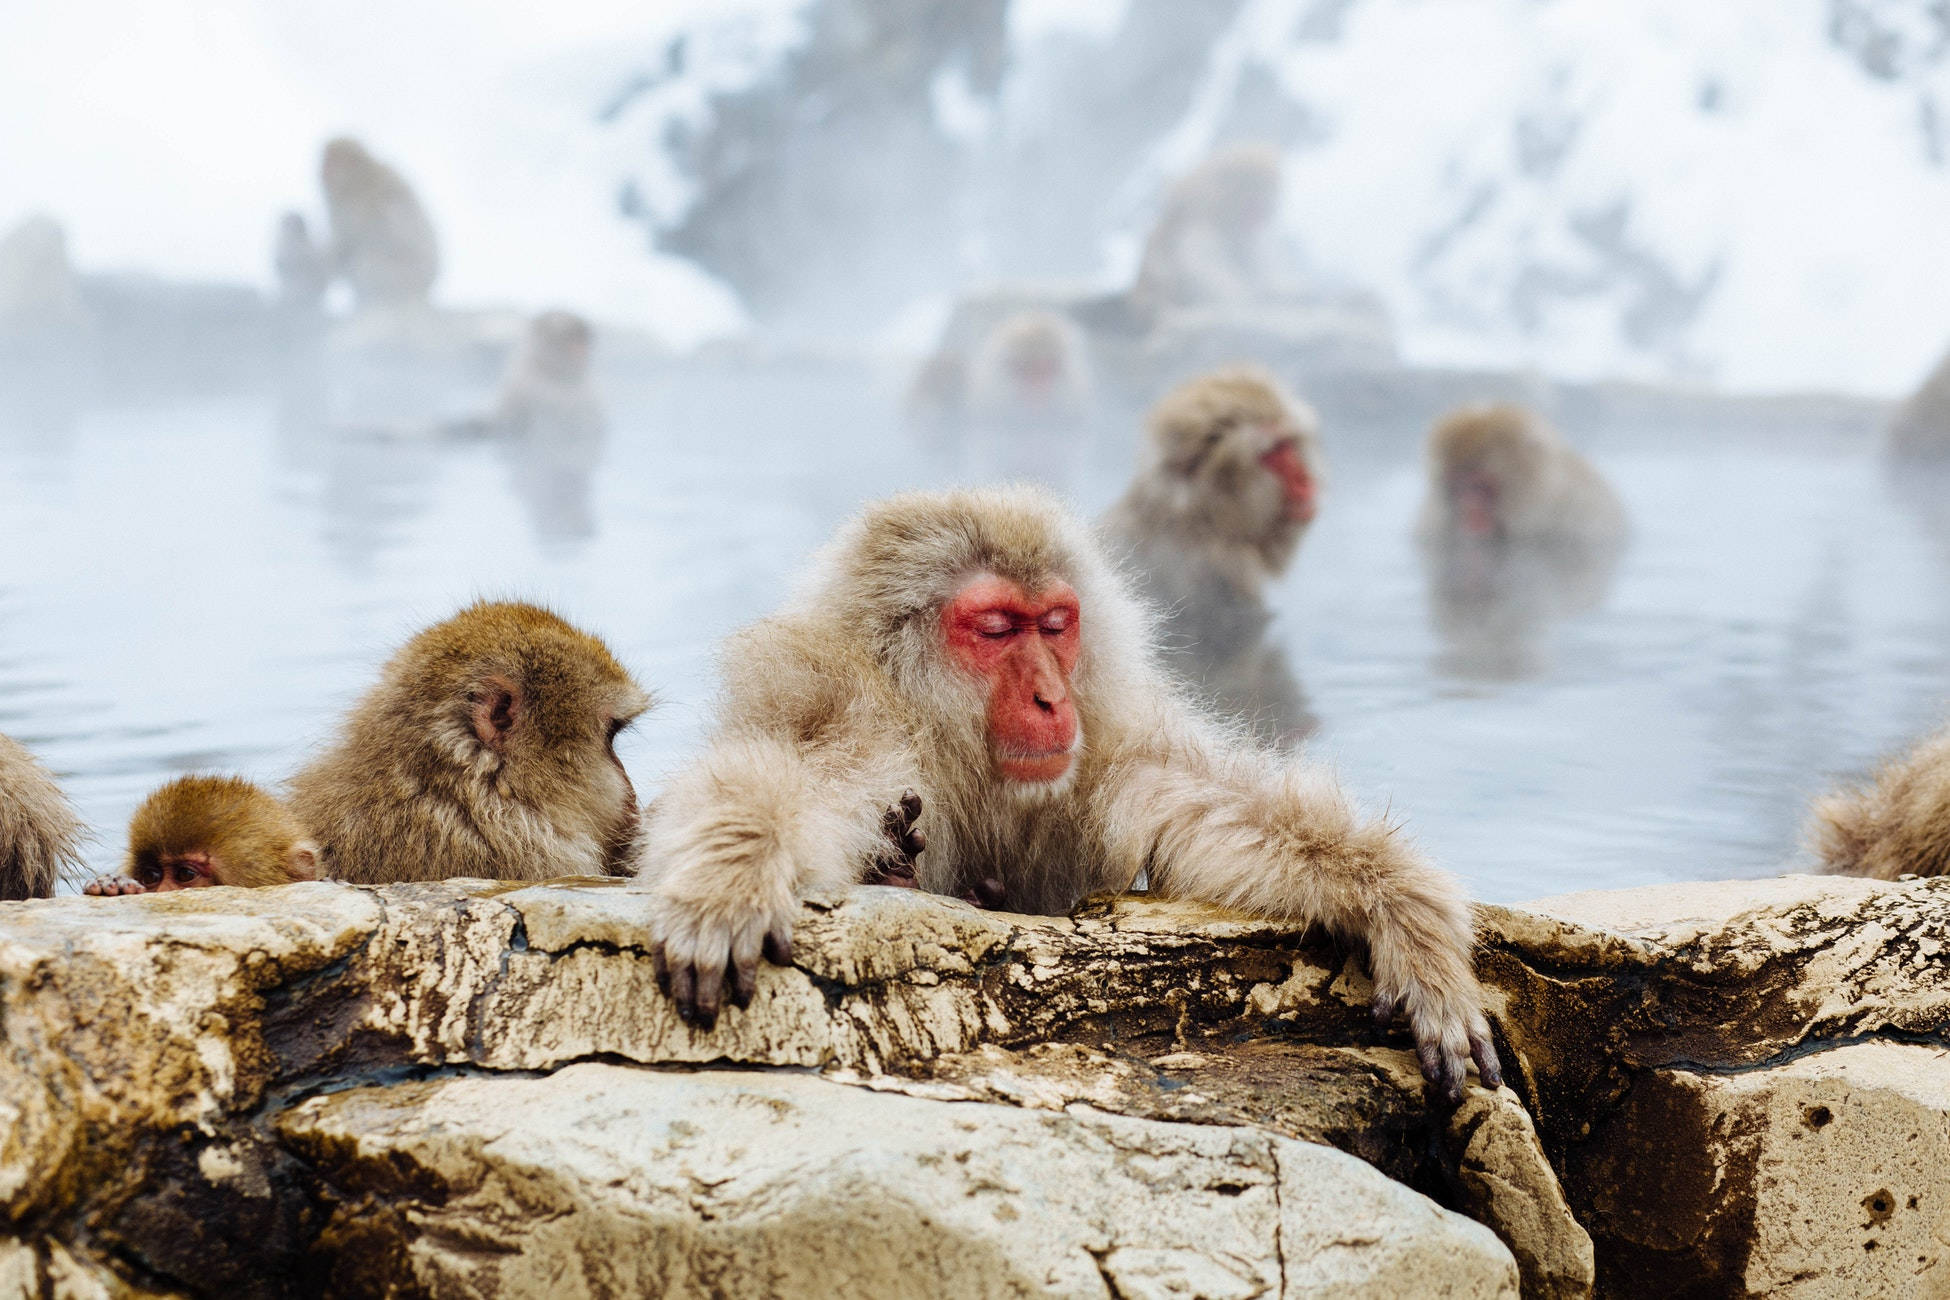
\includegraphics{figures/monkey.jpeg}\\
(Snow Monkey Niseko, Kutchan-chō, Japan)

\section{Report \& presentation}\label{report-presentation}

\textbf{조 구성}\\
- 5인 1조

\textbf{주제}\\
1. 공통: 축산의 가치는 무엇일까? (5분)---식량안보/단백질공급에 대한
내용은 최소화\\
2. \textbf{축산이 국민들에게 사랑받을 수 있는 방법}이 무엇일까?:
구체적인 대안을 고민/발표(15분)\\
3. 어떻게 해야 \textbf{지속가능한 축산이 될 수 있을까?} (15분) or
\textbf{통일에 대비한/통일 후 축산}에 대해서

\textbf{역할}\\
1. 조장: 모든 문제를 조율하고 팀을 잘 이끄는 역할; 공통주제 발표(5분)\\
2. 발표자 1: 주제1에 대한 발표\\
3. 발표자 2: 주제2에 대한 발표\\
4. 기록자 1: 주제 1 내용을 글로 잘 설명 및 제출\\
5. 기록자 2: 주제 2 내용을 글로 잘 설명 및 제출\\
- 발표 및 기록자료 제출: MS word; 발표 당일 09:00까지 email로

\textbf{채점기준}\\
- 주요 기준: 주제에 대해 \textbf{얼마나 고민을 많이 한 흔적이
보이는가?}\\
- 4점: 청중\\
- 4점: 강의자\\
- Total Score: 8/8\\
- 1번째 발표한 조는 심사위원 점수 4점 획득 - 2번째 발표한 조는 심사위원
점수 3\textasciitilde{}4점 획득

\chapter{Introduction}\label{intro}

All living creatures constantly interact with the environment. To
understanding individual animals, we have to understand the relationship
they have with their environment. Also, animals affect the environment.
From birth to death, an animal generates carbon dioxide, methane, feces,
and urine. The excretes from the animal are built with molecules such as
carbon, nitrogen, sulfur, and phosphorus, and are recycled within and
between ecosystems.

\begin{figure}

{\centering 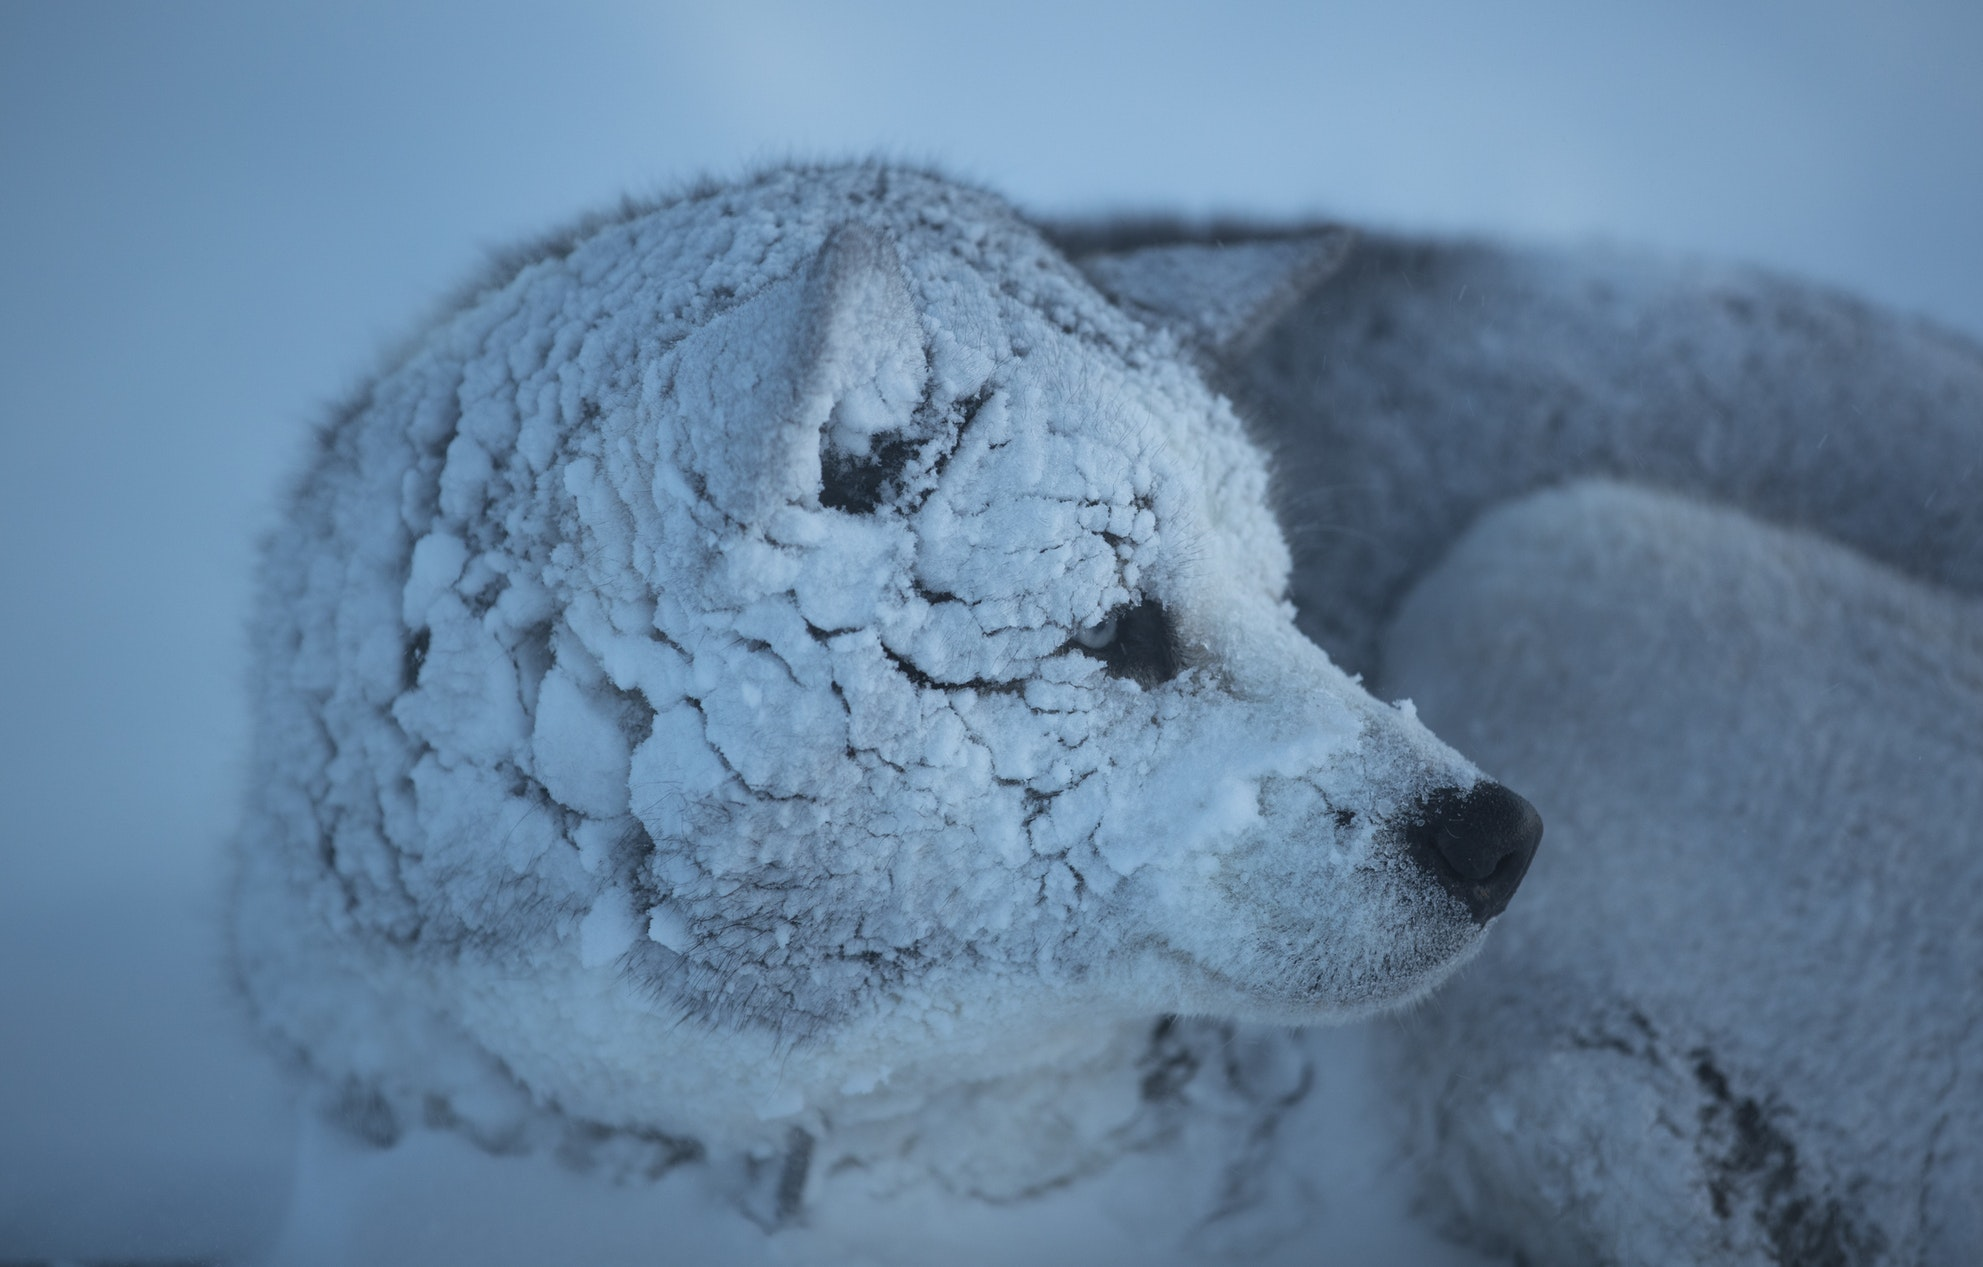
\includegraphics[width=1\linewidth]{figures/polar} 

}

\caption{Alaskan Malamute has the heat-conserving features. To retain heat you want the least body surface area compared to body volume.}\label{fig:snow-dog}
\end{figure}

\chapter{Animal and environment}\label{chapter2}

\textbf{\href{https://youngjunna.github.io/aes/02-AnimalandEnvironment}{강의자료
보기}}

\section{External environment}\label{external-environment}

Animal never separates from the stimuli from outside. Basically, animals
can find food, shelter, protection, and mates from the environment
called \emph{habitat}. The animal habitat includes both phisical
(non-living) and biotic (livinig) components (Table \ref{tab:habitat}).

\begin{table}[t]

\caption{\label{tab:habitat}Components of habitat (physical and biotic)}
\centering
\begin{tabular}{ll}
\toprule
Physical & Biotic\\
\midrule
Temperature & Plant matter\\
Humidity & Predators\\
Oxygen & Parasites\\
Wind & Competitors\\
Soil & Individuals of the same species\\
\addlinespace
Light intensity & \\
Elevation & \\
\bottomrule
\end{tabular}
\end{table}

Animal habitat is constantly changed over time. Not only natural
disasters (eruption of volcano, earthquake, tsunami, and wildfire), also
human activity can affect the animal habitat. Unlike the wildlife, the
environment of domesticated animals (such as cow, pig, poultry, and dog)
that raised in the facility are controlled by the human. In the domestic
animals, the external environment includes both physical (e.g.~housing,
feeder, paddock, fence, and noise) and biotic (e.g.~human, mate, and
feed ingredients) components.

\subsection{Biome}\label{biome}

A biome is a community of plants and animals that have common
characteristics for the environment they exist in (Figure
\ref{fig:biomes}). They can be found over a range of continents. Biomes
are distinct biological communities that have formed in response to a
shared physical climate.

The principal biome-types are:

\begin{enumerate}
\def\labelenumi{\arabic{enumi}.}
\tightlist
\item
  Tundra
\item
  Taiga
\item
  Deciduous forest
\item
  Grasslands
\item
  Desert
\item
  High plateaus
\item
  Tropical forest
\item
  Minor terrestrial biomes
\end{enumerate}

\begin{figure}

{\centering 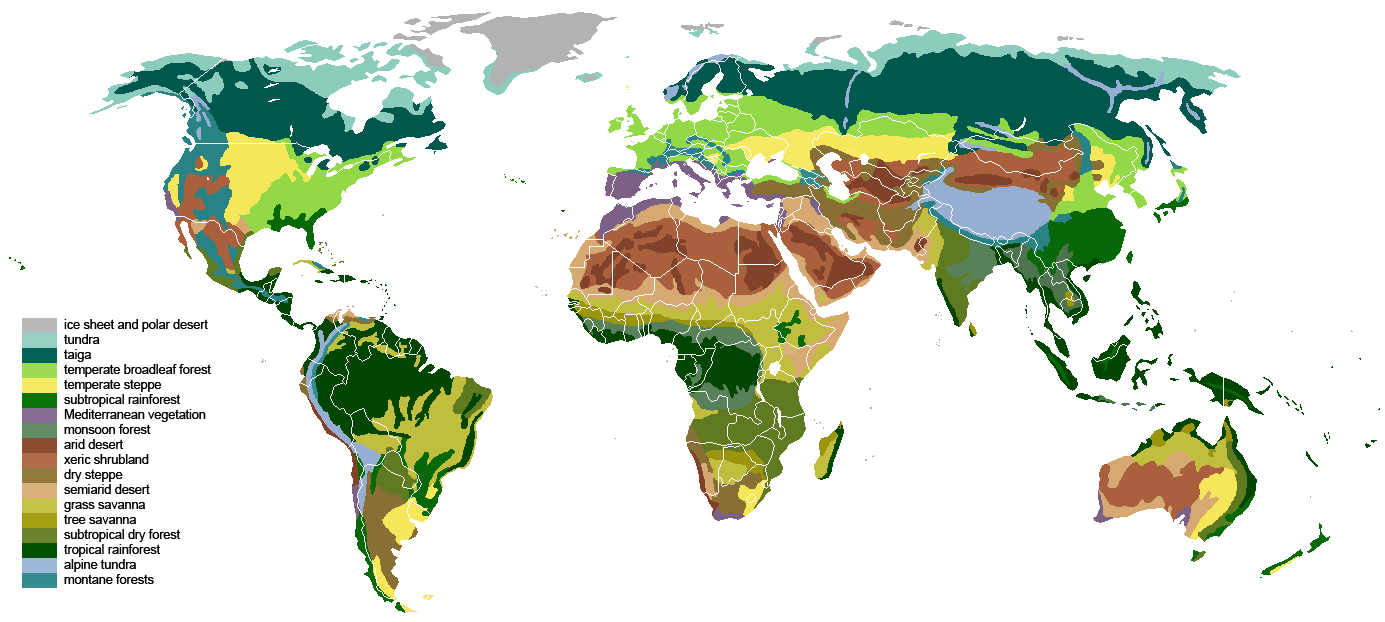
\includegraphics[width=1\linewidth]{figures/biomes} 

}

\caption{Mapping terrestrial biomes around the world}\label{fig:biomes}
\end{figure}

Holdridge (1947; 1967) classified climates based on the biological
effects of temperature and rainfall on vegetation under the assumption
that these two abiotic factors are the largest determinants of the types
of vegetation found in a habitat (Figure \ref{fig:holdridge}).

The three axes of the barycentric subdivisions are:

\begin{enumerate}
\def\labelenumi{\arabic{enumi}.}
\tightlist
\item
  Precipitation (annual, logarithmic)
\item
  Biotemperature (mean annual, logarithmic)
\item
  Potential evapotranspiration ratio (PET) to mean total annual
  precipitation.
\end{enumerate}

Further indicators incorporated into the system are:

\begin{enumerate}
\def\labelenumi{\arabic{enumi}.}
\tightlist
\item
  Humidity provinces
\item
  Latitudinal regions
\item
  Altitudinal belts
\end{enumerate}

\begin{figure}

{\centering 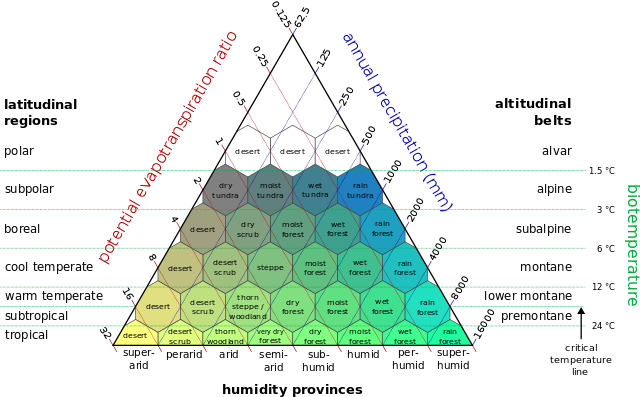
\includegraphics[width=1\linewidth]{figures/lifezones} 

}

\caption{Holdridge life zone classification scheme.}\label{fig:holdridge}
\end{figure}

\section{Internal environment}\label{internal-environment}

\begin{quote}
``The living body, though it has need of the surrounding environment, is
nevertheless relatively independent of it.'' --- Claude Bernard
\end{quote}

Higher animals have complex systems that respond to stimuli to perform
their essential body functions. When the animal receives the signals
from the sensory organs, they produce a local reflex action and/or react
in the central nervous system. Weak signals produce no responses, but
strong stimuli change the physiological or behavioral status of the
animal.

\begin{figure}

{\centering 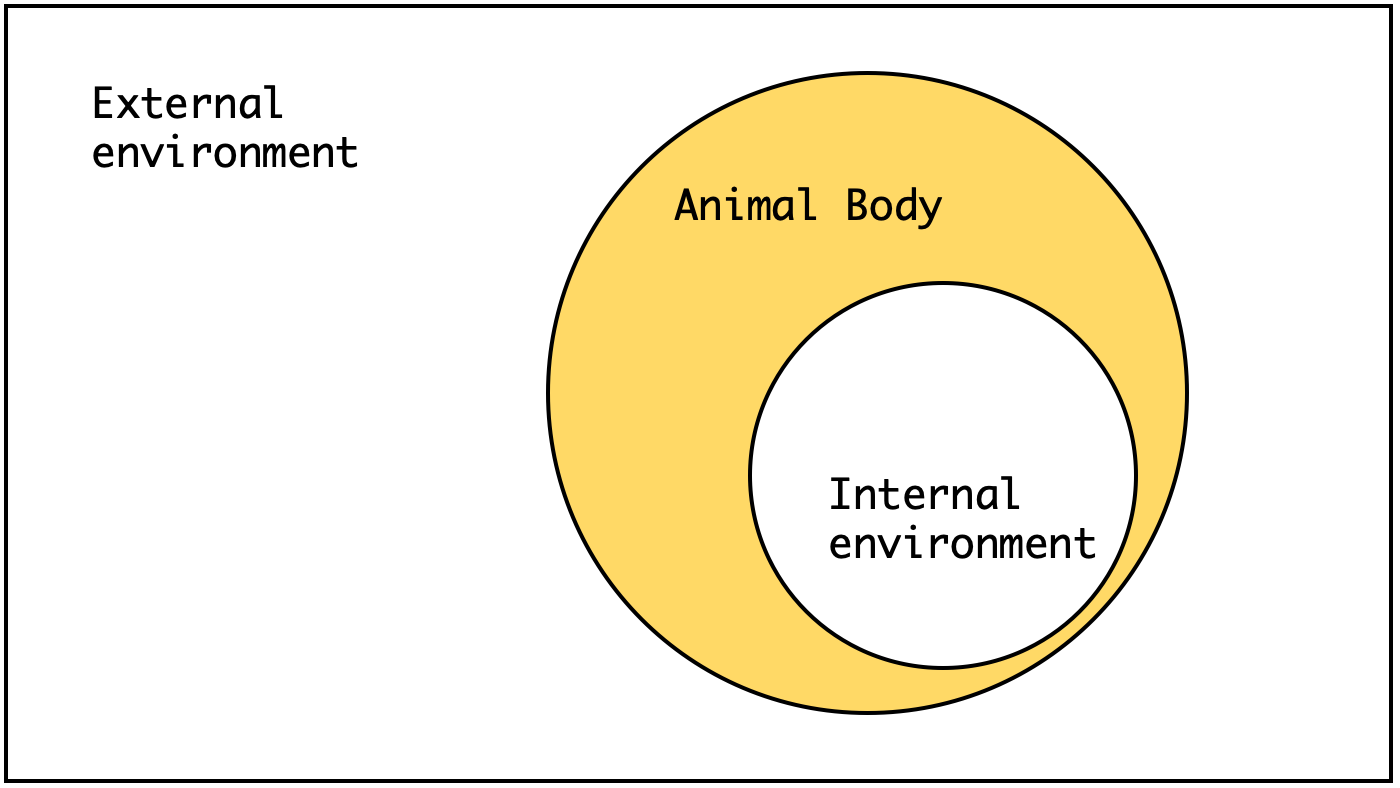
\includegraphics[width=0.6\linewidth]{figures/animal-env} 

}

\caption{External and internal environment}\label{fig:ext-int-env}
\end{figure}

\subsection{Shelford's law of
tolerance}\label{shelfords-law-of-tolerance}

\begin{quote}
``Each and every species is able to exist and reproduce successfully
only within a definite range of environmental conditions.'' --- Ronald
Good
\end{quote}

Although external environments are continuously changed, if animals in
the normal status, they keep the composition of the extracellular fluid
(internal environment) constant to maintain their life. We call it
\emph{homeostasis}.

\begin{table}[t]

\caption{\label{tab:homeostasis}List of homeostatic control variables}
\centering
\begin{tabular}{l}
\toprule
Control variables\\
\midrule
Core temperature; Blood glucose; Iron levels; Copper regulation; Levels of blood gases;\\
Blood oxygen content; Arterial blood pressure; Calcium levels; Sodium concentration;\\
Potassium concentration; Fluid balance; Blood pH; Cerebrospinal fluid; Neurotransmission;\\
Neuroendocrine system; Gene regulation; and Energy balance\\
\bottomrule
\end{tabular}
\end{table}

However, the capacity to maintain the homeostasis is broken when the
animals let the harsh environments and differ by their species.
\textbf{Animals may be limited in their growth and their occurrence by
the minimum, maximum, and optimum condition} \citep{shelford} (Fig.
\ref{fig:law-of-tol}).

\begin{figure}

{\centering 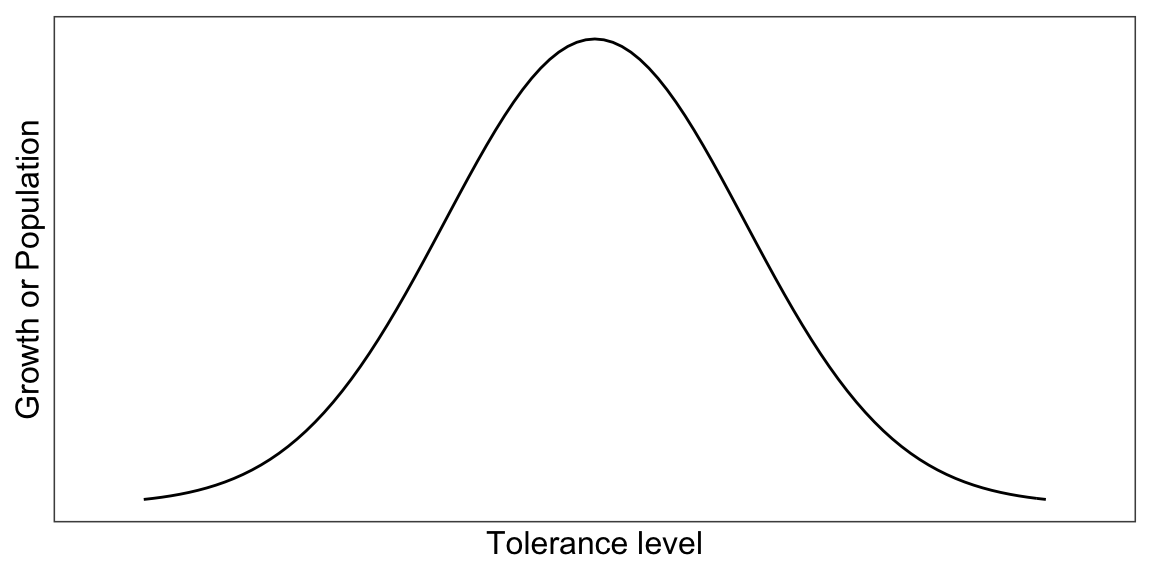
\includegraphics{AES_files/figure-latex/law-of-tol-1} 

}

\caption{Shelford's law of tolerance}\label{fig:law-of-tol}
\end{figure}

The optimum range of environmental condition may differ within the same
organism, and it is not necessarily fixed. They can change as:

\begin{itemize}
\tightlist
\item
  Change of seasons
\item
  Change of environmental conditions
\item
  Life stage of the organism
\end{itemize}

\subsection{Adaptation}\label{adaptation}

\begin{quote}
``Changes in morphological, anatomical, physiological, biochemical and
behavioral characteristics of the animal which promote welfare and favor
survival in a specific environment.'' --- Hafez
\end{quote}

\citet{hafez1968adaptation} defined an adaptation as above. The
adaptation helps an animal survive in their external environment. The
representative adaptive traits are:

\begin{enumerate}
\def\labelenumi{\arabic{enumi}.}
\tightlist
\item
  Structural adaptation
\item
  Behavioral adaptation
\item
  Physiological adaptation
\end{enumerate}

Structural adaptation is the changes in physical features (e.g.~body
shape, skin, and internal organs) of the animal. Behavioral adaptation
is the changes in behaviors (e.g.~searching for food, mating,
vocalizations, and mitigation) of the animal. Physiological adaptation
is the changes in the animal body functions such as growth, temperature
regulation, and ionic balance. Sometimes, adapted animal create a new
species (\emph{speciation}).

\begin{figure}

{\centering 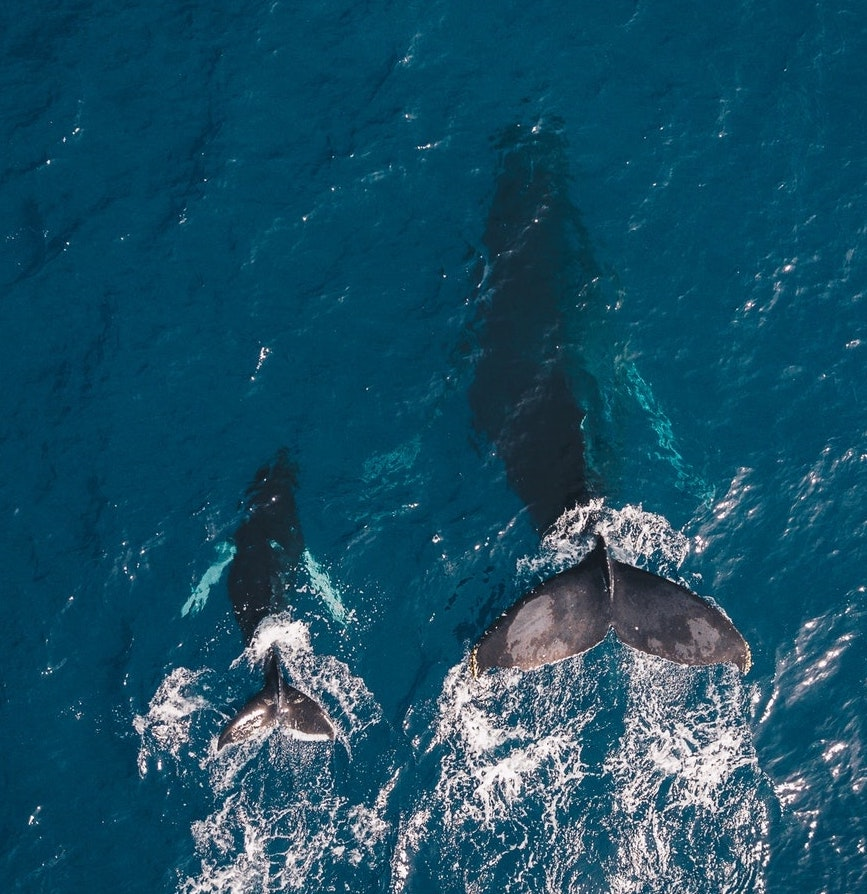
\includegraphics[width=1\linewidth]{figures/adaptation} 

}

\caption{Migration is an example of a behavioral adaptation. Grey whales swim from the Arctic to Mexico every year.}\label{fig:adaptation}
\end{figure}

\subsection{Acclimatization}\label{acclimatization}

Acclimatization is the physiological changes induced by a complex of
factors such as altitude, temperature, humidity, photoperiod, or pH.
Acclimatization is the short-term process (hours to weeks) by comparison
with adaptation (take place over many generations).

\chapter{Temperature}\label{temperature}

\textbf{\href{https://youngjunna.github.io/aes/03-Temperature}{강의자료
보기}}

Temperature is a quantity expressing of the amount of heat. Because a
rate of every chemical reaction occurs in the animal's body is affected
by the temperature, it is a very important factor to all animals. Like
most chemical reactions, an enzyme-catalyzed reaction rate in the
animal's body increases as the temperature is raised. However, extremely
high or low temperature results in loss of activity or lose the
structure for most enzymes (\emph{denaturation}; Figure \ref{fig:q10}).

\begin{figure}

{\centering 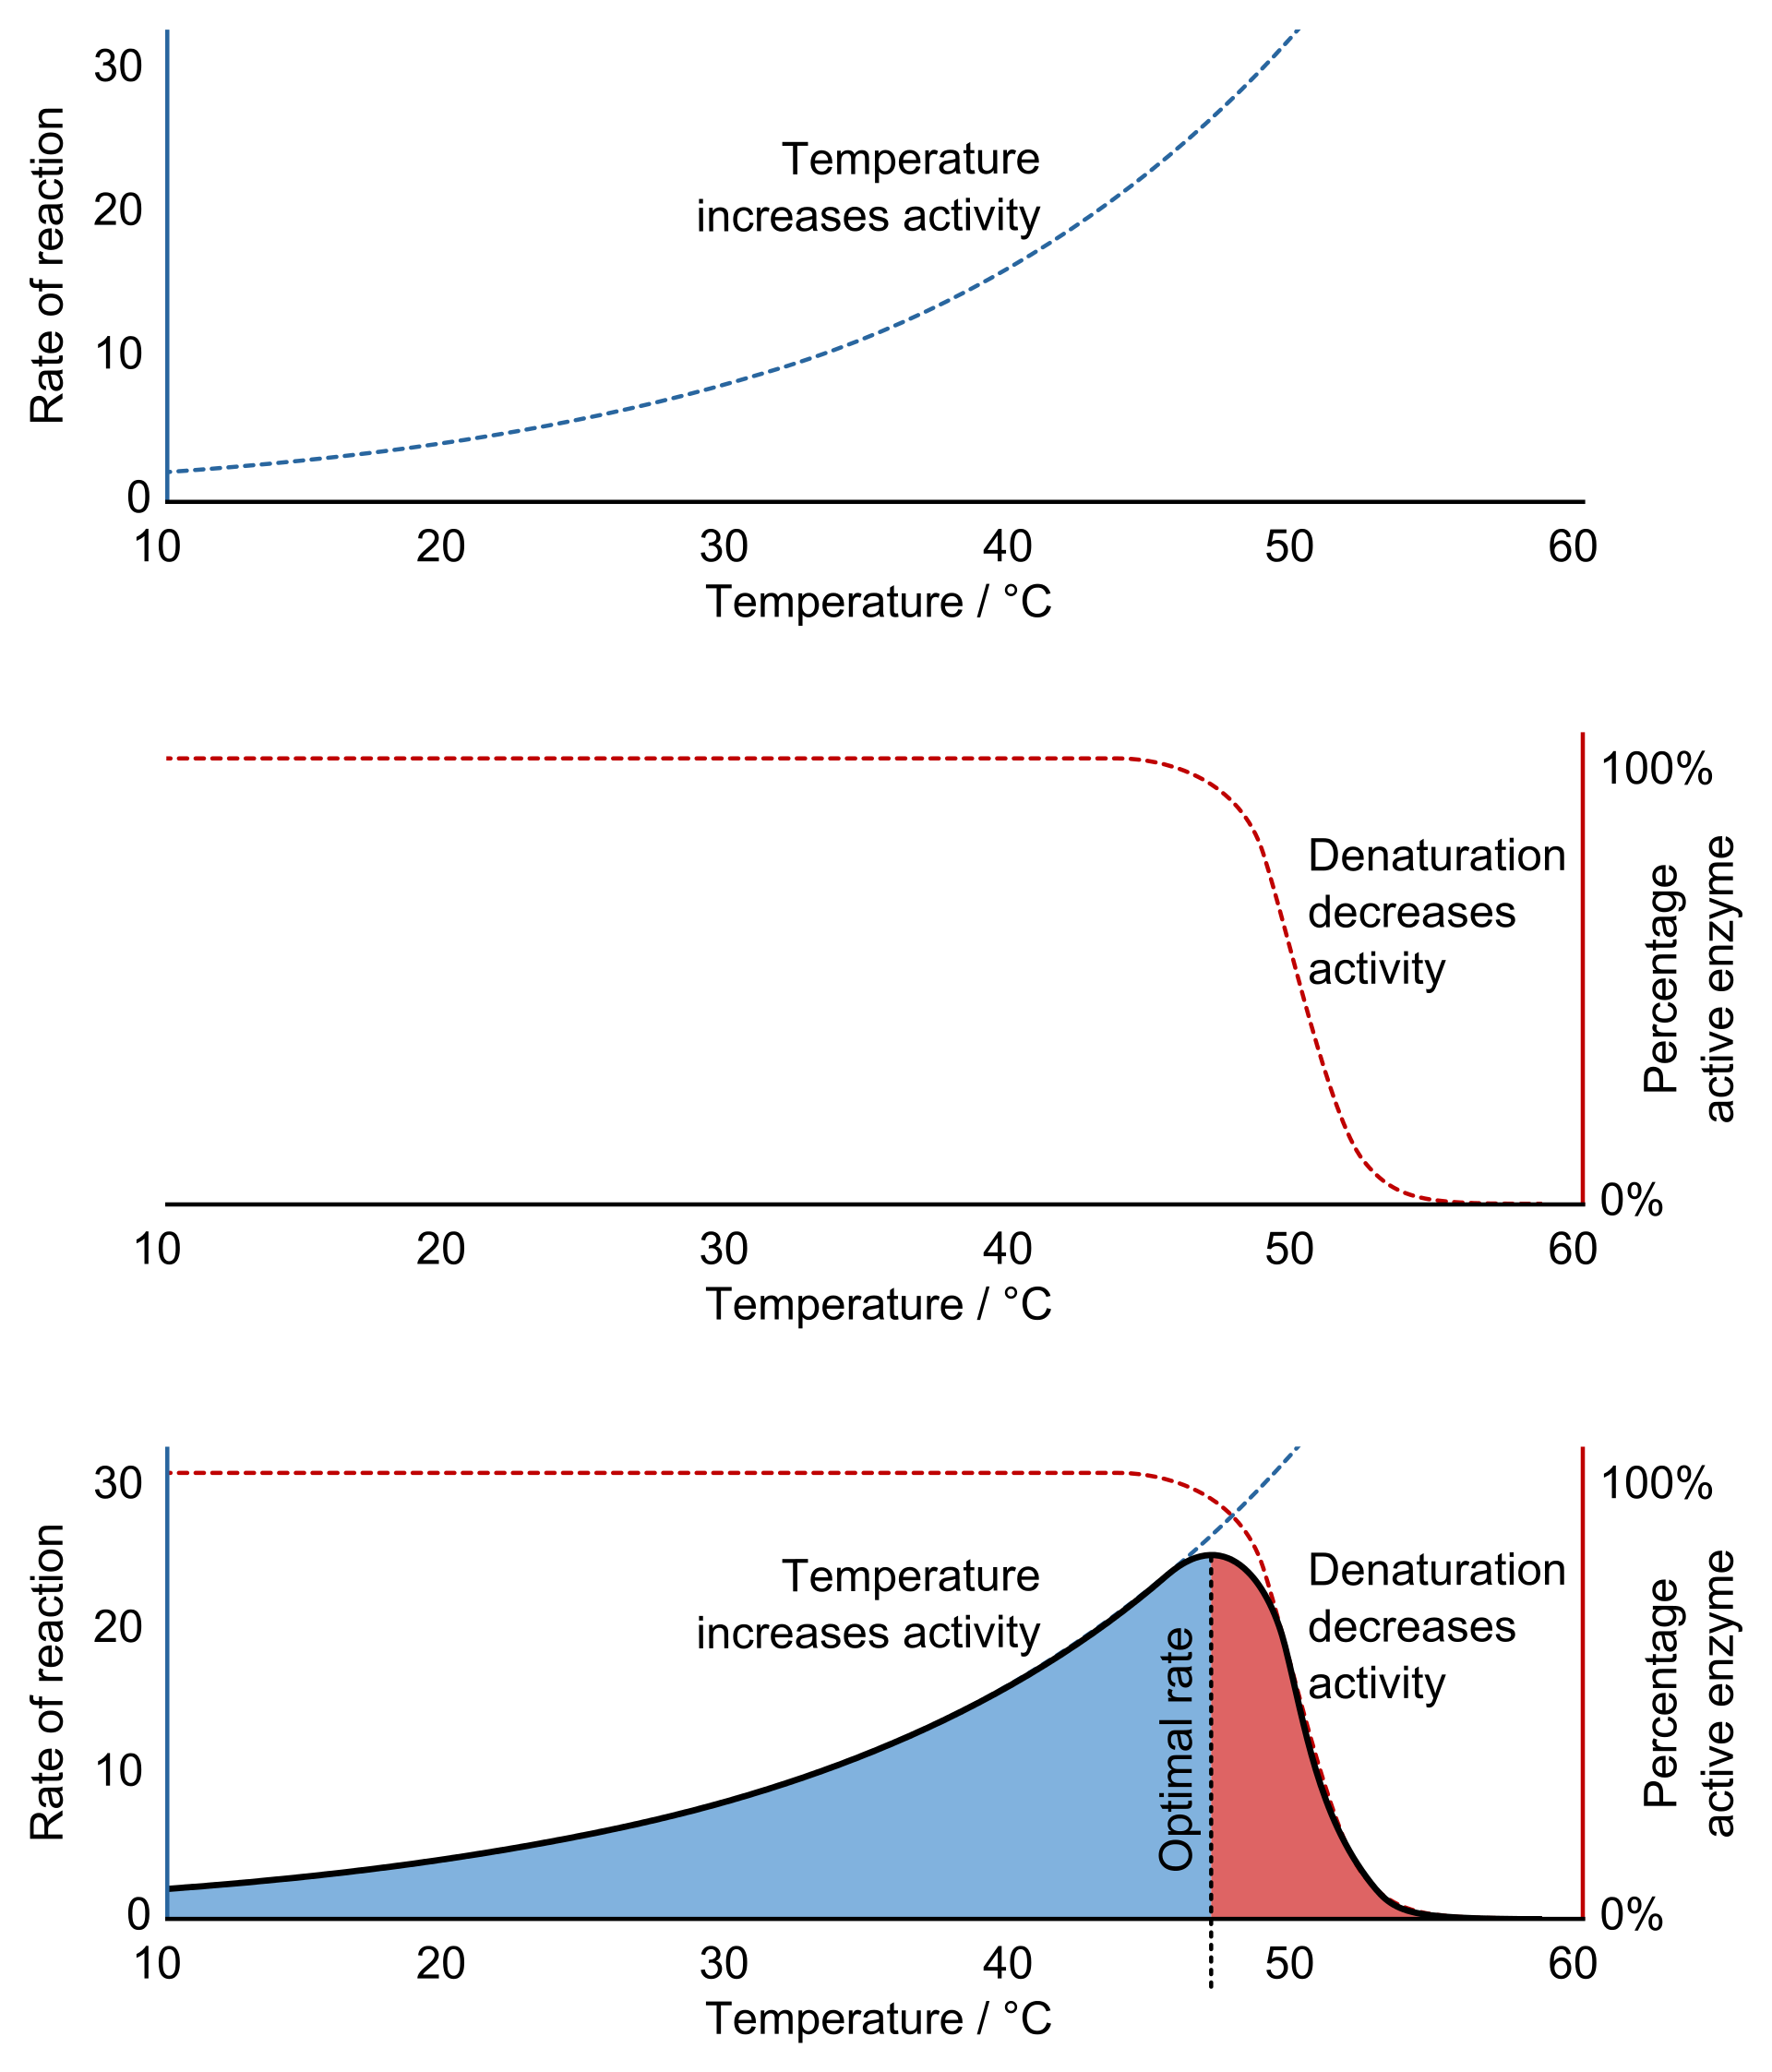
\includegraphics[width=0.6\linewidth]{figures/q10} 

}

\caption{The effects of temperature on enzyme activity [@q10]. Top - increasing temperature increases the rate of reaction (Q10 coefficient). Middle - the fraction of folded and functional enzyme decreases above its denaturation temperature. Bottom - consequently, an enzyme's optimal rate of reaction is at an intermediate temperature.}\label{fig:q10}
\end{figure}

\section{Poikilotherm and homeotherm}\label{poikilotherm-and-homeotherm}

Key factors for animal surviving are to adapt to external environmental
changes and maintain a consistent internal environment. The animal can
be divided into two types for response to external temperatures:
\emph{poikilotherm} (cold-blooded animals) and \emph{homeotherm}
(warm-blooded animals). Examples of poikilotherms are most fish,
amphibians, and reptiles. Their internal body temperature varies
considerably according to their external environments. On the other
hand, homeotherm maintains their thermal homeostasis regardless of the
external temperature. The examples of homeotherm are birds and mammals.

\begin{figure}

{\centering 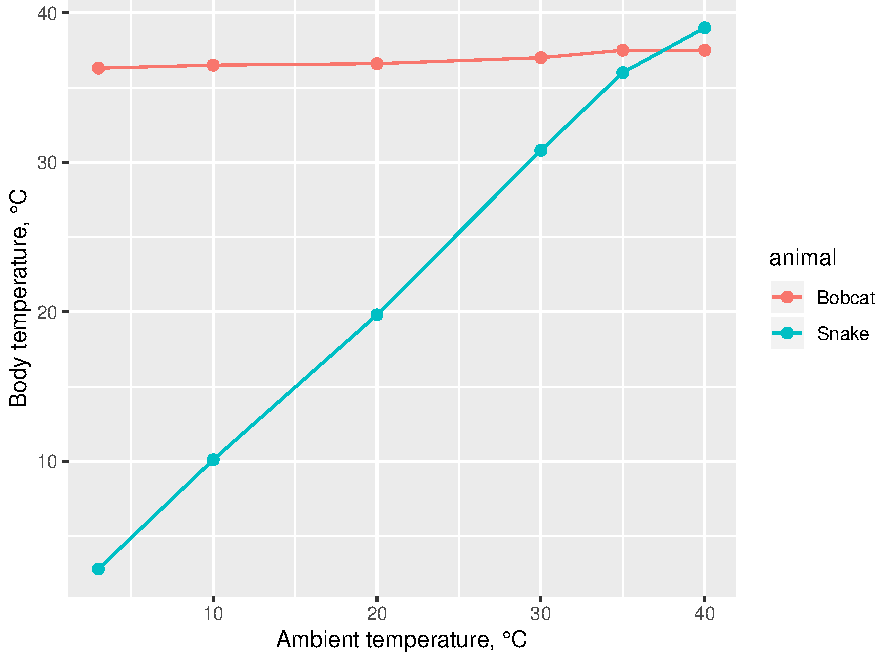
\includegraphics{AES_files/figure-latex/body-temp-comparision-1} 

}

\caption{Comparison of body temperature response by snake (poikiloterm) and bobcat (homeoterm) to changing ambient temperature.}\label{fig:body-temp-comparision}
\end{figure}

\subsection{Poikilotherm}\label{poikilotherm}

The term derives from the acient Greek language \emph{poikilos}
(ποικίλος; changeable) and \emph{thermos} (θερμός; heat). The body
temperature of poikilotherms varies considerably than those of
homeotherms (Figure \ref{fig:body-temp-comparision}). They generally use
solar radiation for maintaining their body temperature and have four to
ten enzyme systems that can operate at different ambient temperature
because the temperature affects the chemical reactions.

\begin{figure}

{\centering 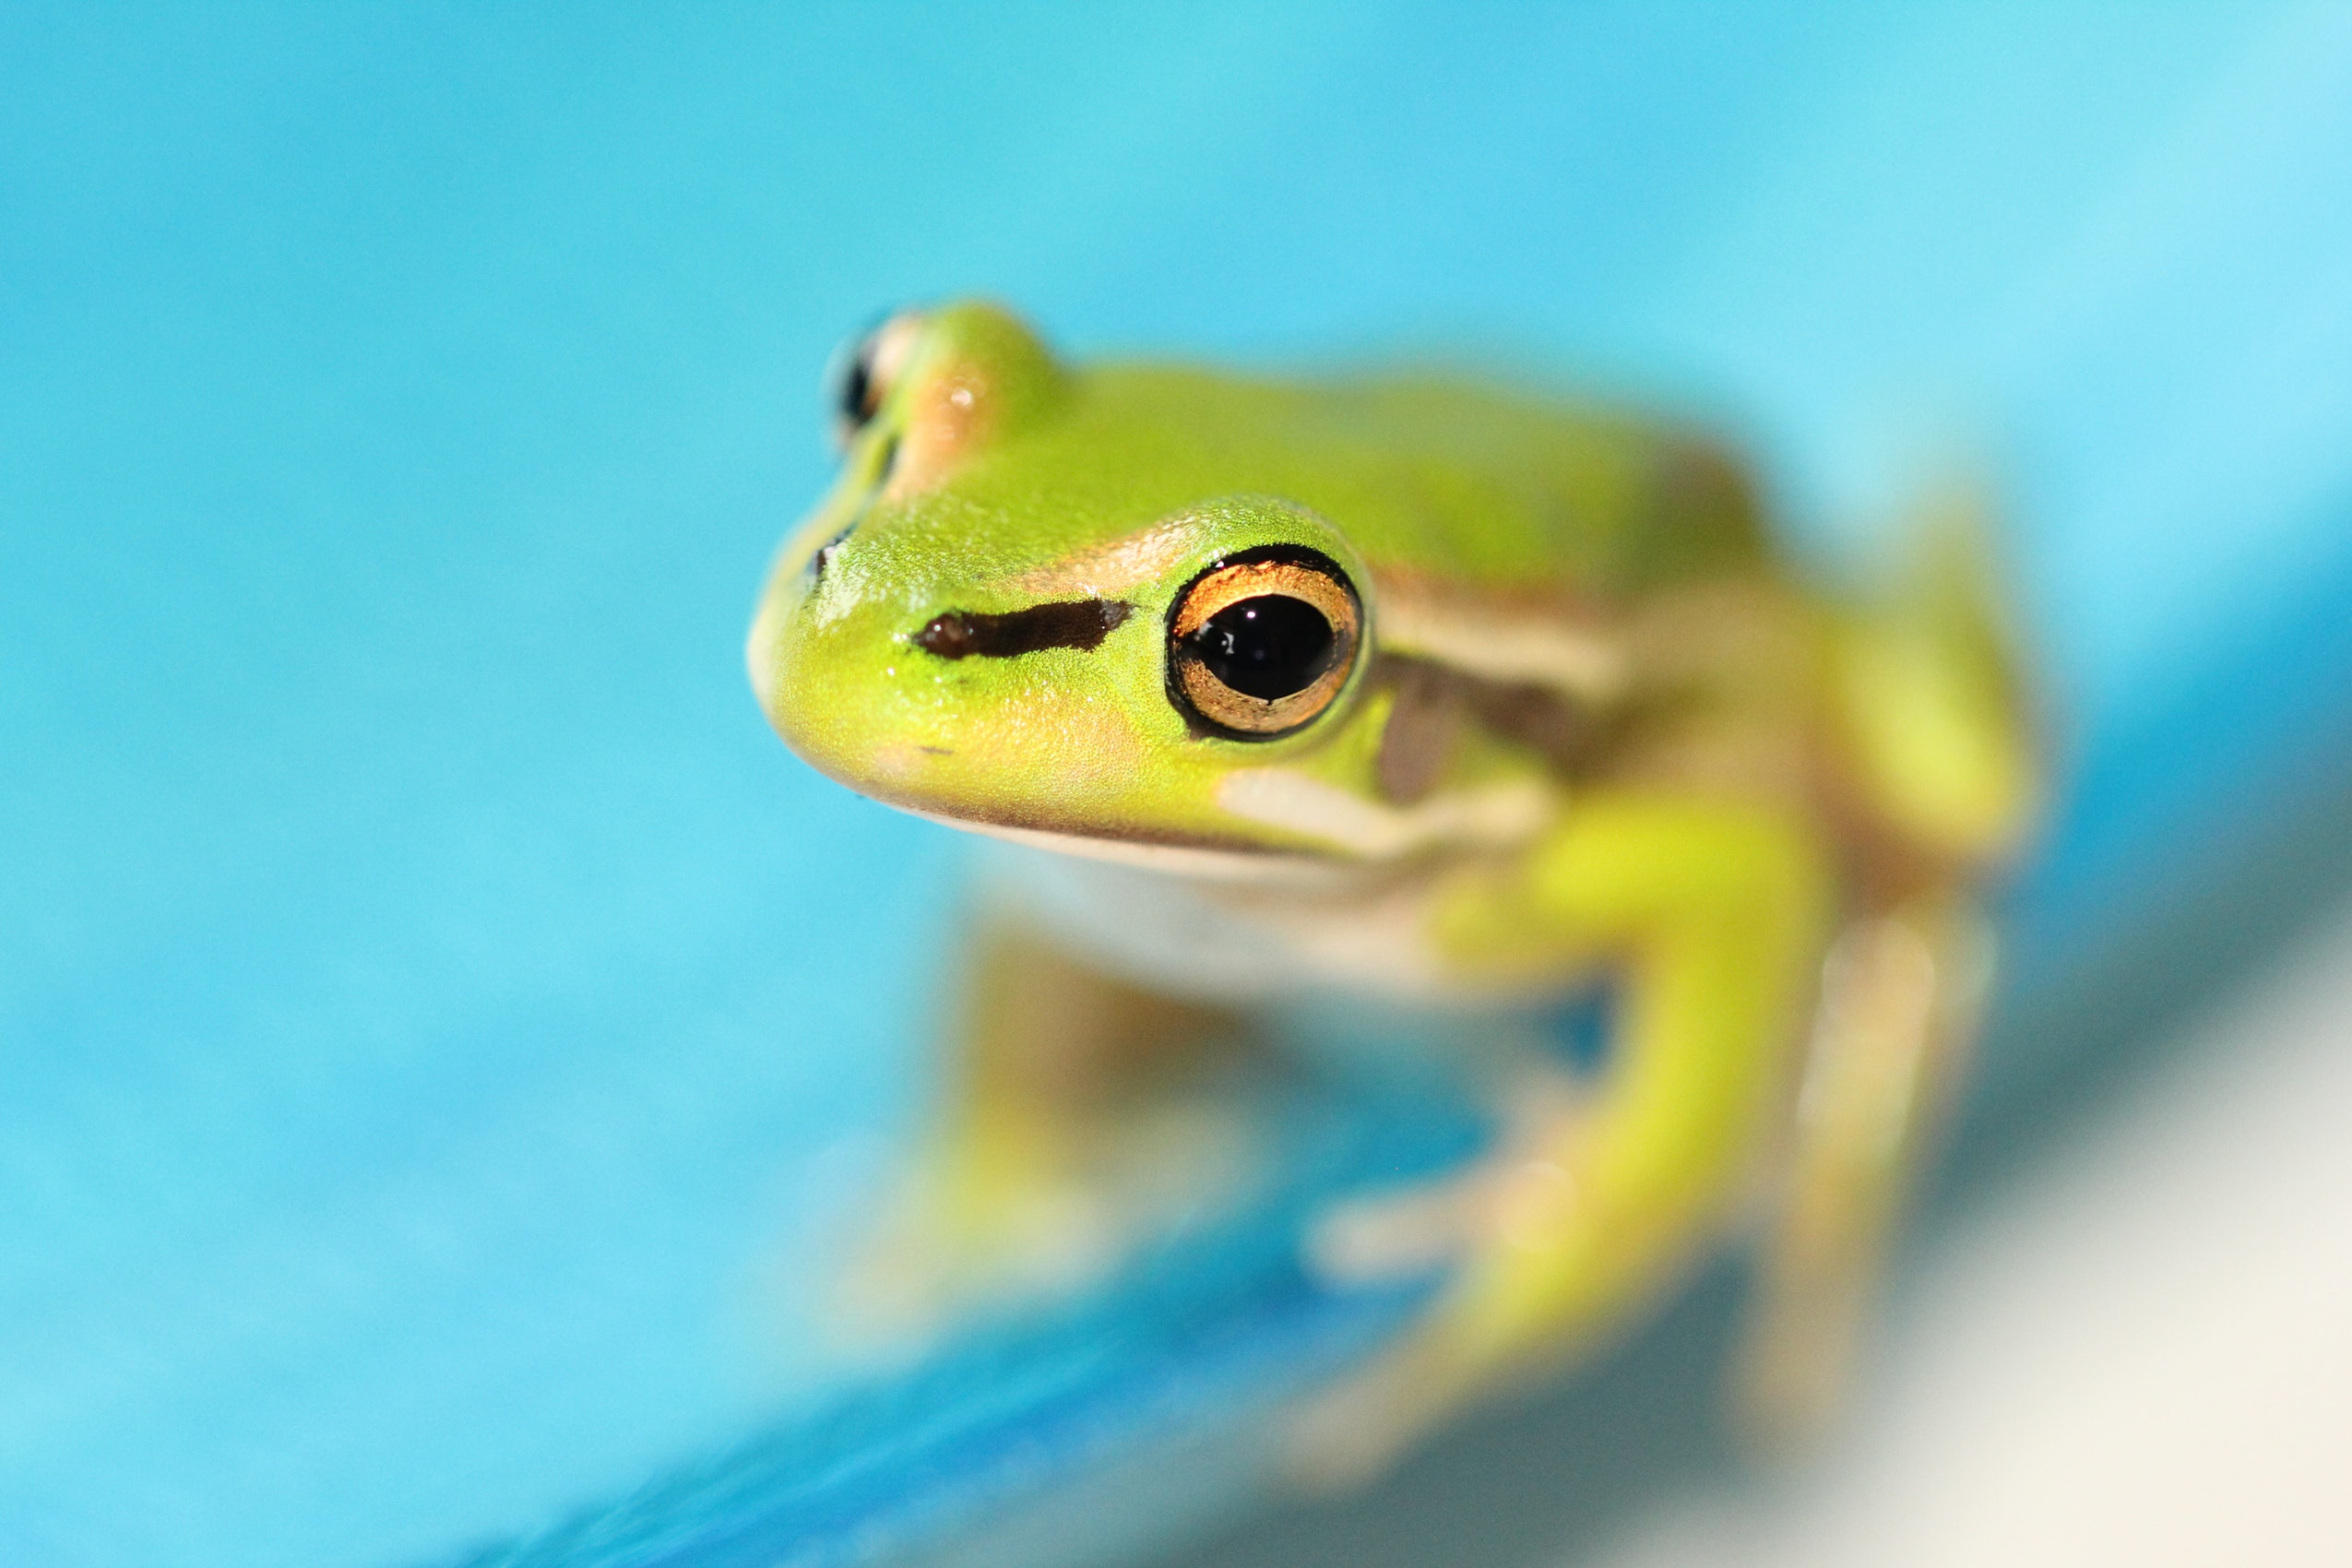
\includegraphics[width=1\linewidth]{figures/flog} 

}

\caption{Green frog on blue surface.}\label{fig:flor}
\end{figure}

\subsection{Homeoterm}\label{homeoterm}

Homeotherms can maintain body temperature independently from ambient
temperatures by regulating the metabolic process. They preserve their
body temperature by muscle contraction and brown adipose tissue is
catabolized for heat production \citep{grigg2004evolution}. In hot
environments, they use evaporative cooling (sweating or panting) for
maintaining their body temperature. Most of the domestic animals are
homeotherm.

\begin{figure}

{\centering 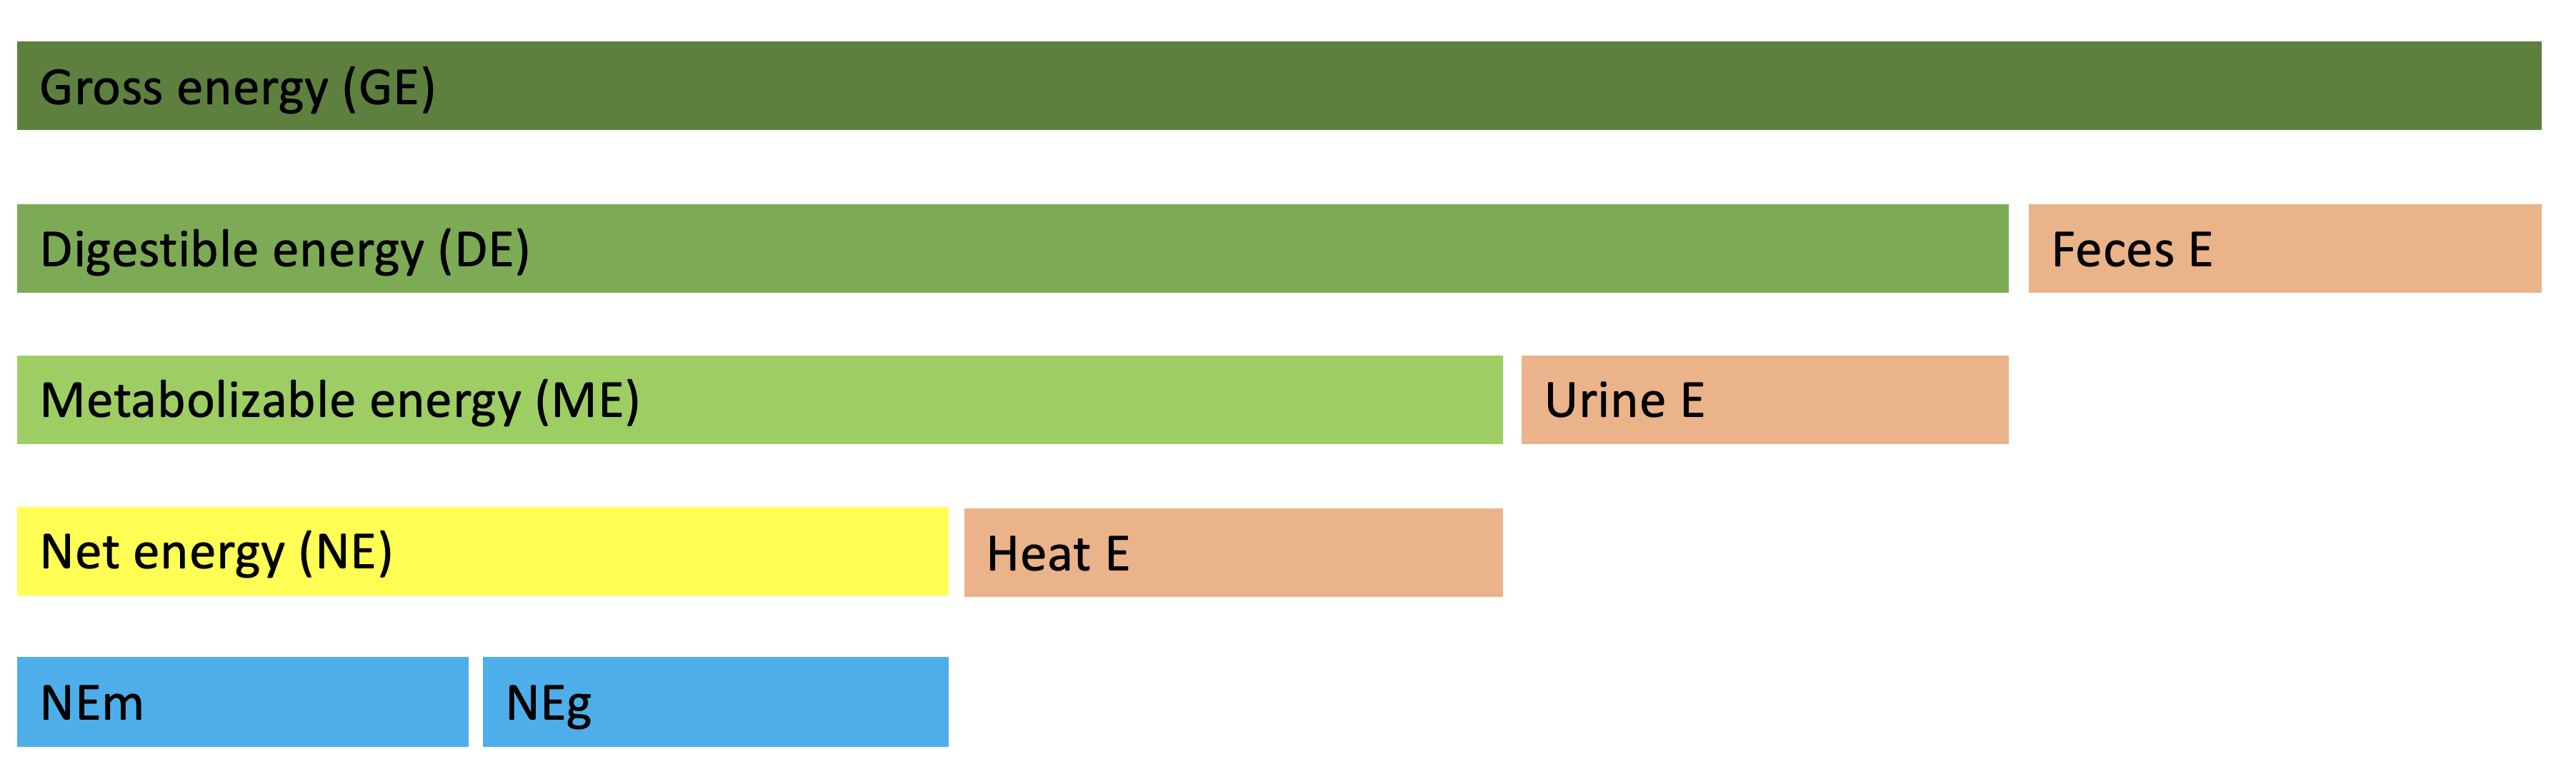
\includegraphics[width=1\linewidth]{figures/energy-system} 

}

\caption{Overview of feed energy flow through the animal body}\label{fig:e-system}
\end{figure}

\begin{figure}

{\centering 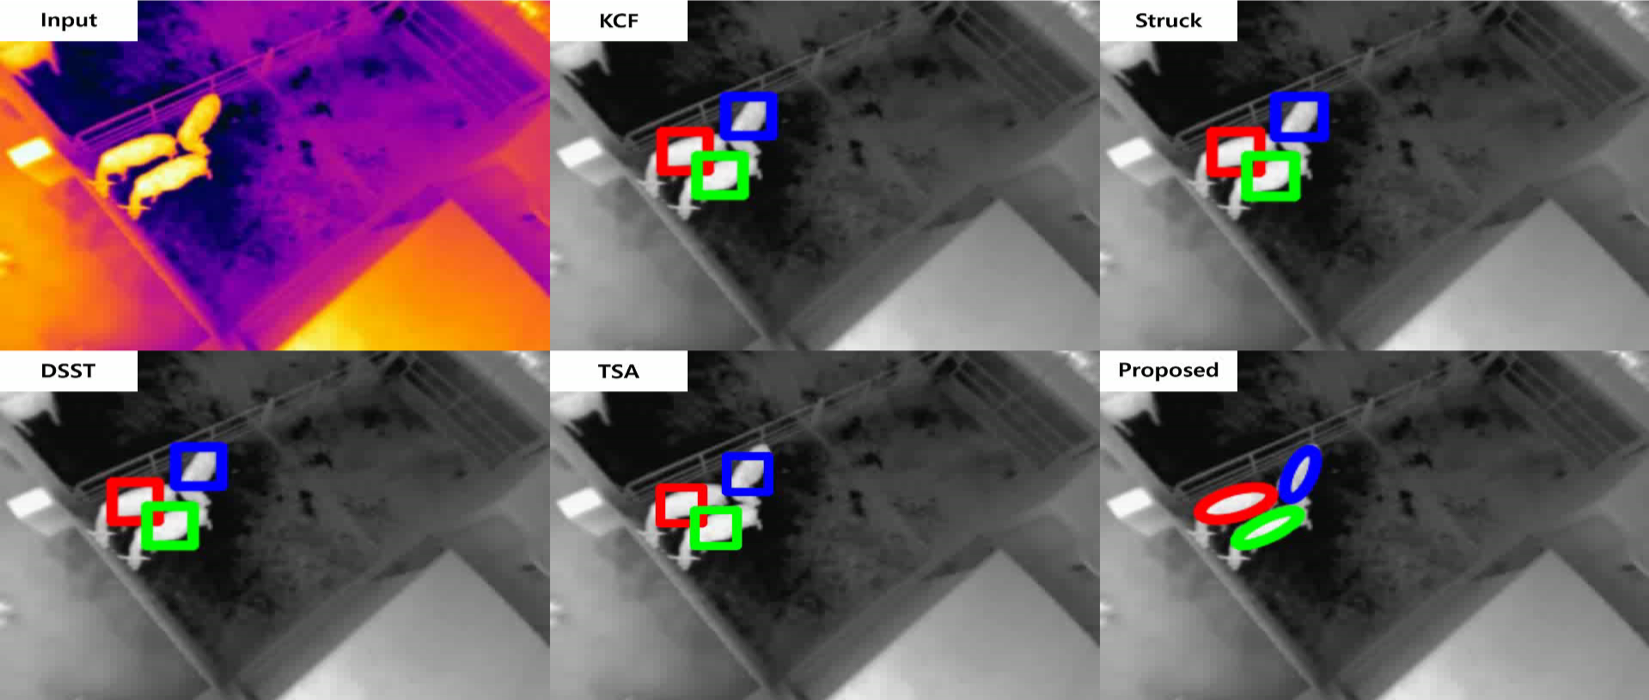
\includegraphics[width=1\linewidth]{figures/kimetal} 

}

\caption{Infrared cameras image that cows generating the heats. @kim2018image developed the algorithms for tracking the cows using IR camera video.}\label{fig:kimetal}
\end{figure}

In some homeoterms (bears, hedgehog, marmot, and so on) and
poikilotherms (frogs, turtles, snake, and so on), they can enter the
\emph{hibernation} in the cold season: the body temperature is dropped,
and the metabolic rate is depressed. Hibernating bears can recycle their
body proteins and urine to avoid muscle loss.

\subsection{Heterotherm}\label{heterotherm}

Heterotherms exhibit the characteristics of both poikilotherm and
homeotherm. They can switch between poikilothermic and homeothermic
strategies. In some bat species, for example, body temperature and
metabolic rate are elevated only when they are active. When they at
rest, metabolic rate is drastically dropped thereby the body temperature
is decreased to the ambient temperature.

\section{Thermoregulation}\label{thermoregulation}

Thermoregulation is a process to maintain the internal temperature
within certain boundaries. In homeotherms, thermoregulatory physiology
is mainly controlled by nervous and endocrine systems. The core
temperature of the animal is primarily regulated by the hypothalamus. If
the ambient temperature is going to cold, they generate heat via
metabolic processes to keep their body temperature. In contrast, in hot
conditions, sweat glands release sweat for evaporates and the blood
vessels going to wider for increasing the blood flow to the skin.

\begin{table}[t]

\caption{\label{tab:norm-body-temp}Normal body temperature of the domestic animals; Body temperatures may be 1°C above or below these temperatures.}
\centering
\begin{tabular}{llll}
\toprule
Animal & Normal temperature (°C) & Animal & Normal temerature (°C)\\
\midrule
Cattle & 38.5 & Donkey & 38.2\\
Calf & 39.5 & Chicken & 42.0\\
Buffalo & 38.2 & Camel & 34.5-41.0\\
Sheep & 39.0 & Horse & 38.0\\
Llama, alpaca & 38.0 & Pig & 39.0\\
\addlinespace
Goat & 39.5 & Piglet & 39.8\\
\bottomrule
\end{tabular}
\end{table}

In poikilotherms, they use external sources of temperature to keep their
body temperatures (Table \ref{tab:cooling}). To regulate their body
temperature, they sometimes climbing the trees, entering the warm water,
lying on the cool ground, or lying in the sun. There are some methods
for thermoregulation in poikilotherms: \emph{convection},
\emph{conduction}, and \emph{radiation}. Convection is the transfer of
heat via the movement of molecules within fluids (gases or liquids).
Conduction is the transfer of heat via the direct molecular collision.
Radiation is the transfer of heat in the form of waves or particles
(sunlight is the most familiar forms of radiation). Once there's a
thermal equilibrium between the animal and environment, the thermal
exchange will be stopped.

\begin{table}[t]

\caption{\label{tab:cooling}Cooling and heating methods for poikilotherms}
\centering
\begin{tabular}{lll}
\toprule
Methods & Cooling & Heating\\
\midrule
Convection & Increasing blood flow to body surfaces & Entering a warm water or air current; Building an insulated nest or burrow\\
Conduction & Lying on cool ground; Staying wet in a river, lake or sea; Covering in cool mud & Lying on a hot surface\\
Radiation & Get away from the sun & Lying in the sun; Folding skin to reduce exposure\\
\bottomrule
\end{tabular}
\end{table}

\section{Temperature humidity index
(THI)}\label{temperature-humidity-index-thi}

The productivity of domestic animals is primarily affected by air
temperature, and altered by wind, humidity, and radiation.
Temperature--humidity index (THI) is a combination of temperature and
humidity that is a measure of the degree of discomfort experienced by an
individual in warm weather (a.k.a. discomfort index). This unitless
index was first introduced by Thom (1959) to describe the effect of
ambient temperature on humans but has been adapted to describe thermal
conditions that drive heat stress in dairy cattle (De Rensis et al.,
2015). Temperature-humidity index for dairy cow is calculated as

\(THI = (0.8*T) + [H*(T - 14.4)] + 46.4\)

where T is the air temperature and H is the relative humidity. The THI
is a useful tool for predicting the heat stress of cows, however, it
does not account for solar radiation and wind speed which can affect the
heat load of cattle.

\begin{figure}

{\centering 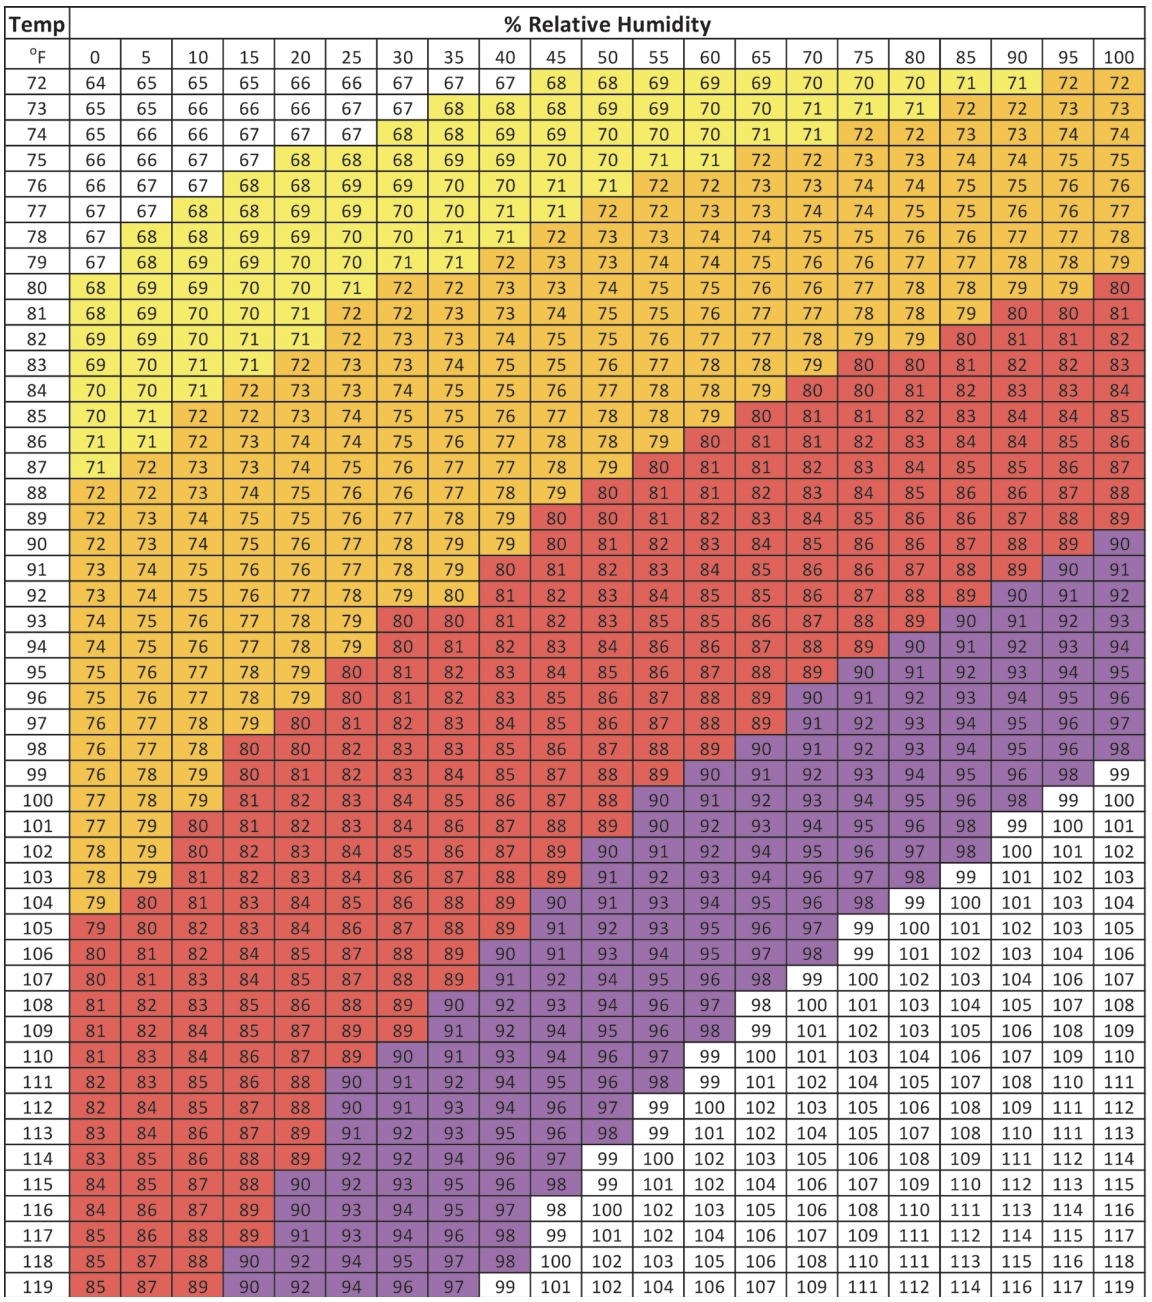
\includegraphics[width=1\linewidth]{figures/THI} 

}

\caption{THI chart for dairy cows. Yellow = Stress Threshold Respiration rate exceeds 60 BPM. Milk yield losses begin. Repro losses detectable. Rectal Temperature exceeds 38.5°C (101.3°F). Orange = Mild-Moderate Stress Respiration Rate Exceeds 75 BPM. Rectal Temperature exceeds 39°C (102.2°F). Red = Moderate-Severe Stress Respiration Rate Exceeds 85 BPM Rectal Temperature exceeds 40 °C (104°F). Purple = Severe Stress. Respiration Rate 120-140 BPM. Rectal Temperature exceeds 41 °C (106°F)}\label{fig:THI}
\end{figure}

\section{Effects heat stress on the animal production and
health}\label{effects-heat-stress-on-the-animal-production-and-health}

Homeotherms have optimal temperature zones for production within which
no additional energy above maintenance is expended to heat or cool the
body. The range for lactating dairy cows is estimated to be from −0.5 to
20°C (Johnson, 1987).

\subsection{Dairy cattle}\label{dairy-cattle}

\begin{figure}

{\centering 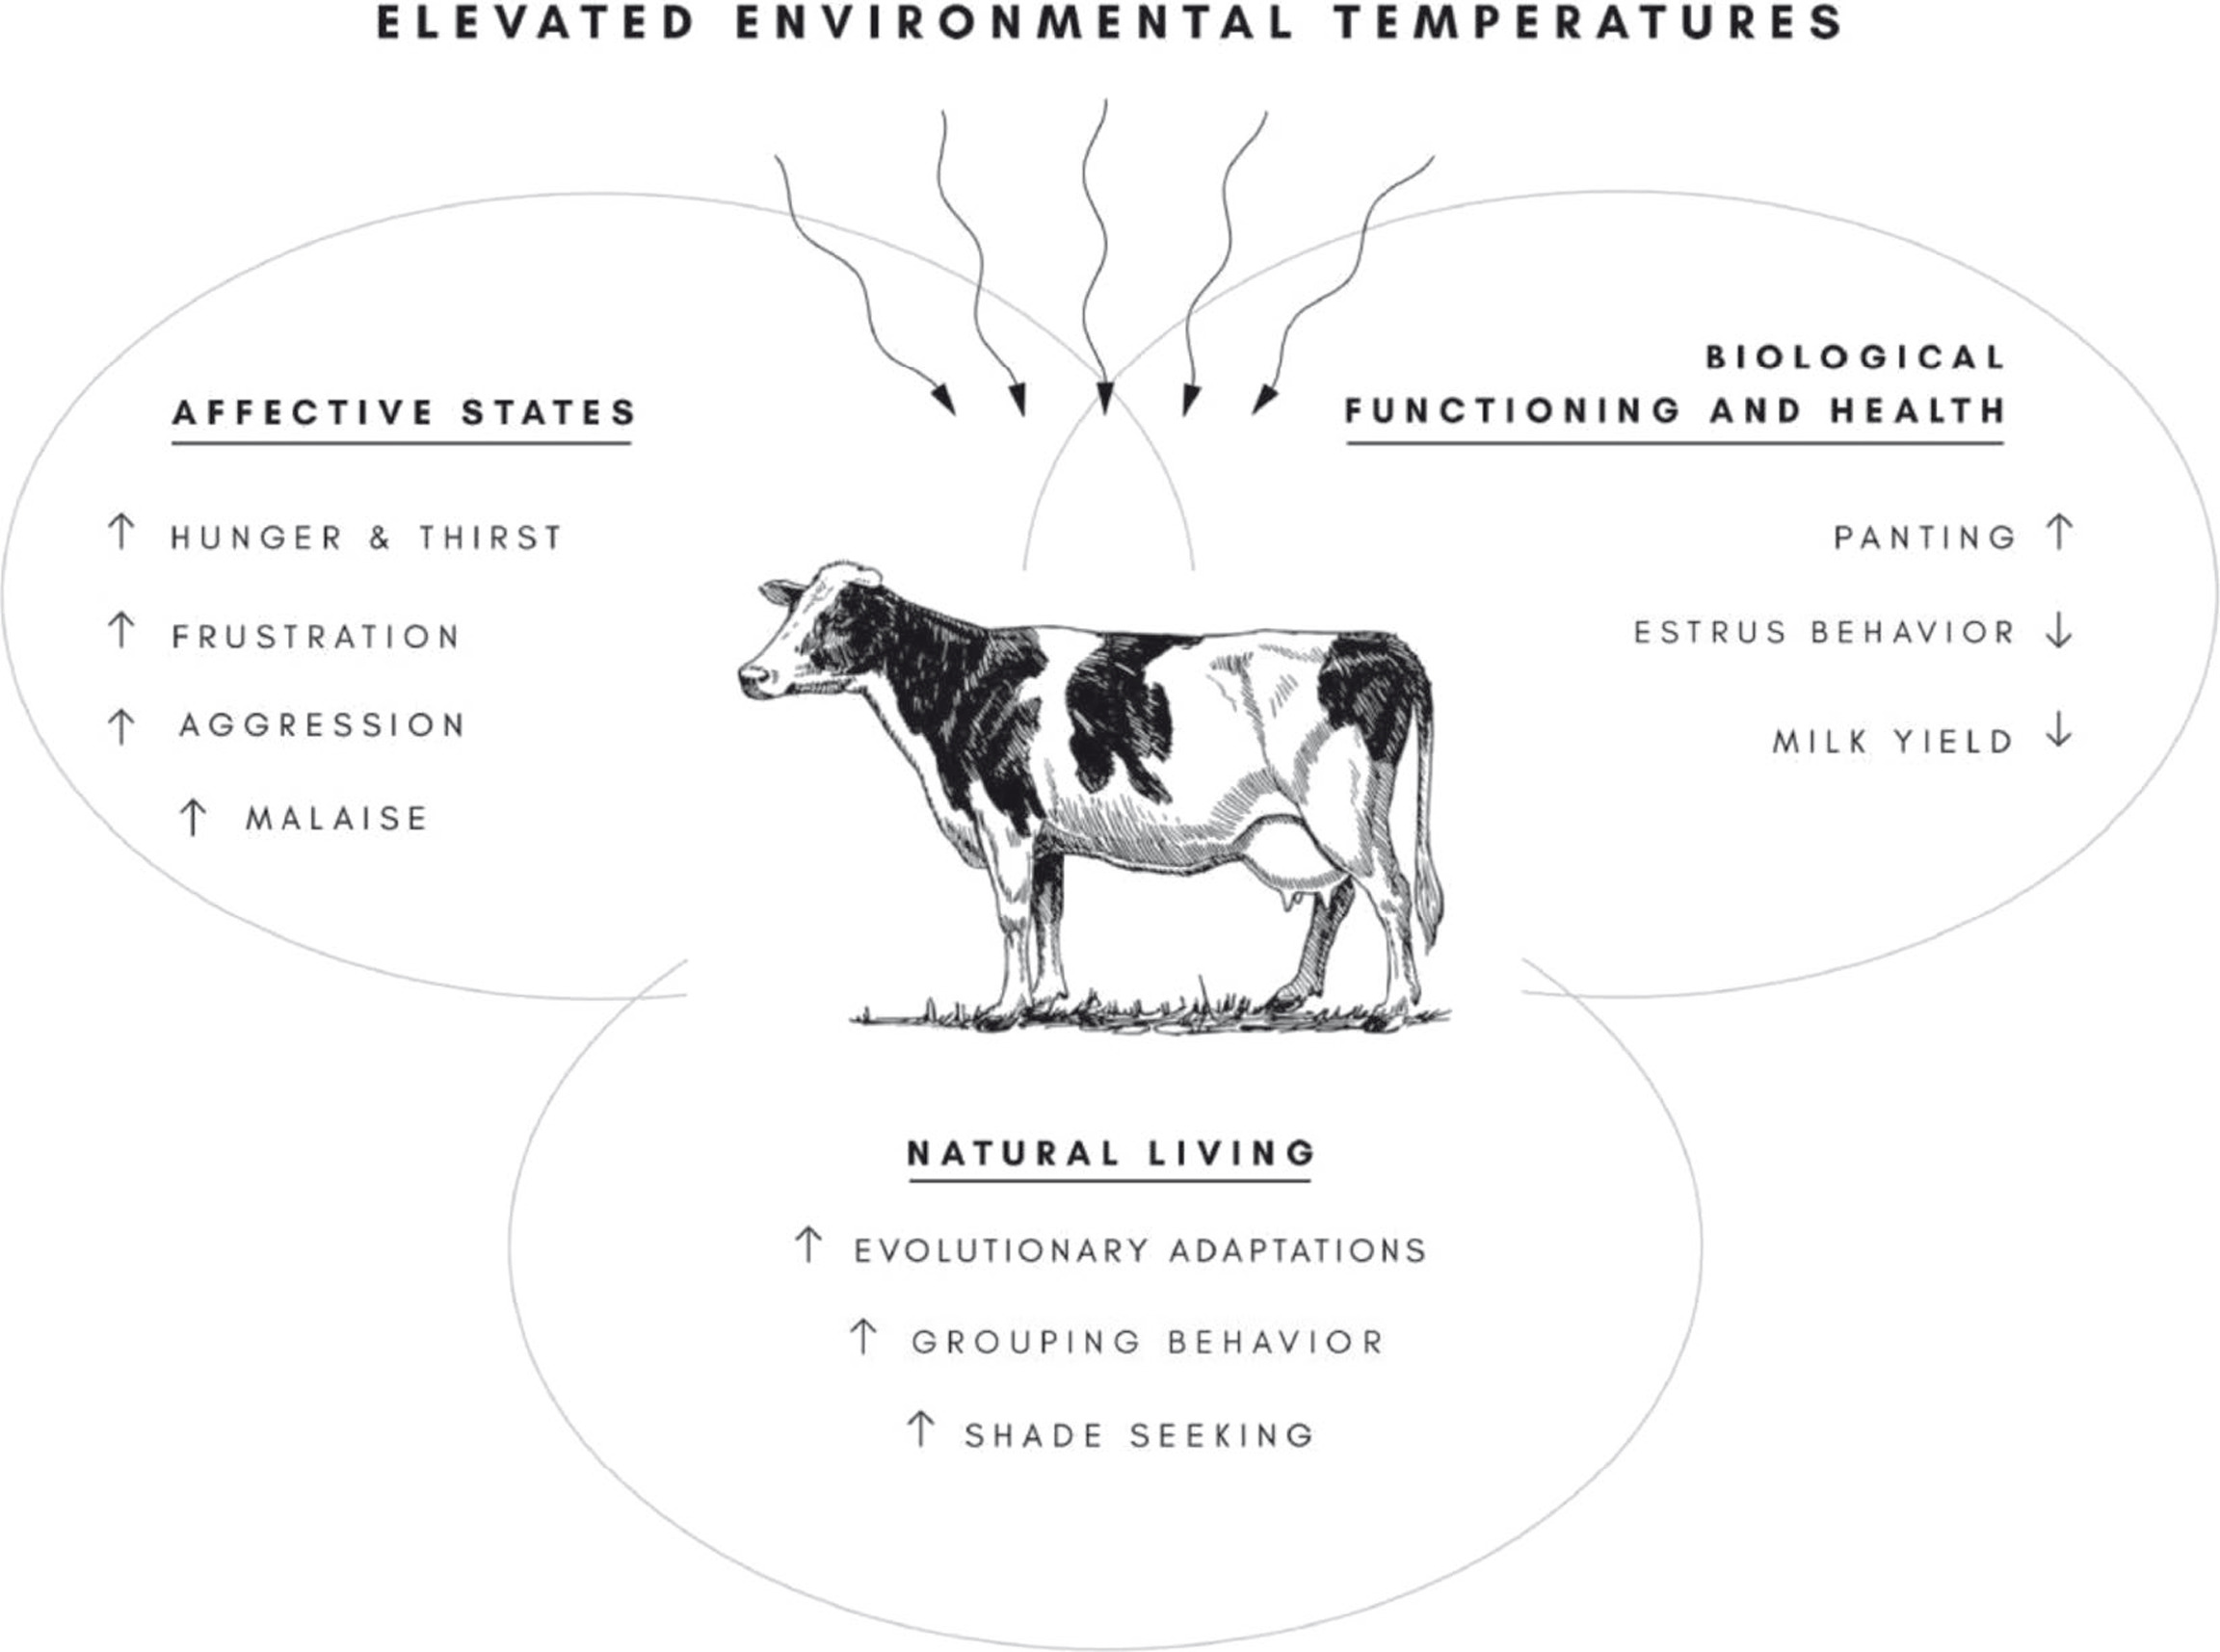
\includegraphics[width=1\linewidth]{figures/heatstress-dairy} 

}

\caption{The relationship between the immediate effects of environmental heat stress and the 3 key constructs of animal welfare: (1) the biological functioning (and health) of the animal, (2) the affective states the animal is experiencing, and (3) the naturalness of its life under current heat management strategies (Polsky et al., 2017).}\label{fig:heat-dairy}
\end{figure}

\textbf{Heat stress decreases milk production.} Lactating dairy cows
have an increased sensitivity to heat stress compared with nonlactating
(dry) cows, due to milk production elevating metabolism (Purwanto et
al., 1990). Moreover, because of the positive relationship between milk
yield and heat production, higher yielding cows are more challenged by
heat stress than lower yielding animals (Spiers et al., 2004).

When a cow becomes heat stressed, an immediate coping mechanism is to
reduce DMI, causing a decrease in the availability of nutrients used for
milk synthesis (West, 2003; Rhoads et al., 2009). Simultaneously, there
is an increase in basal metabolism caused by activation of the
thermoregulatory system. Mild to severe heat stress can increase
metabolic maintenance requirements by 7 to 25\% (NRC, 2001).

\textbf{Heat stress decreases reproductivity}. The decrease in
conception rates during summer seasons can range between 20 and 30\%,
with evident seasonal patterns of estrus detection (De Rensis and
Scaramuzzi, 2003). Elevated environmental temperatures negatively affect
the cow's ability to display natural mating behavior, as it reduces both
the duration and intensity of estrous expression (Orihuela, 2000). A
reduction in estrous behavior has been argued to be the result of
reduced DMI and the subsequent effects on hormone production (Westwood
et al., 2002). Decreased milk production and declining reproductive
success are the most commonly examined components of a heat-stressed
dairy cow's health.

Alterations in housing and management strategies have attempted to
mitigate the heat stress. Basically, various cooling options for dairy
cows exist based on the principles of convection, conduction, radiation,
and evaporation.

\begin{enumerate}
\def\labelenumi{\arabic{enumi}.}
\item
  \textbf{Fan installations}, which facilitate air movement and increase
  convection, have been used to reduce environmental temperatures and
  mitigate heat stress by decreasing respiratory rate and rectal
  temperature and increasing DMI (Armstrong, 1994).
\item
  \textbf{High-pressure mist injected into fans} (which function to cool
  the microclimate air that the cows inspire) or large water droplets
  from low-pressure sprinkler systems that completely wet the cow by
  soaking the hair coat.
\item
  \textbf{Physical structures} that provide shade such as trees, roofs,
  or cloth can create more hospitable microclimates for cows because of
  the reduction in solar radiation exposure and decline in ambient
  temperature.
\item
  \textbf{Barn orientation} (depending on geographic location) can also
  help mitigate heat stress by reducing the insolation and stall surface
  temperature.
\end{enumerate}

\subsection{Beef cattle}\label{beef-cattle}

As temperatures heat up during the summer cattle producers need to
assess the heat stress that their cattle are under. Typically pastured
cattle are not as susceptible to heat stress as feedlot cattle. Pastured
cattle have the ability to seek shade, water and air movement to cool
themselves.

Compared to other animals cattle cannot dissipate their heat load very
effectively. Cattle do not sweat effectively and rely on respiration to
cool themselves. Cattle should not be worked during times of extreme
heat and only early in morning when it is hot.

Cattle's core temperature peaks 2 hours after peak environmental
temperature. It also takes at least 6 hours for cattle to dissipate
their heat load. Therefore, if peak temperature occurred at 4:00 pm
cattle will not have recovered from that heat load until after 12:00 am
and it will be later than that before cattle have fully recovered from
the entire days heat load. Special attention should be paid to cattle
with increased risk of heat stress including heavy cattle, black cattle
and respiratory compromised animals.

\subsubsection{Heat stress management}\label{heat-stress-management}

\begin{enumerate}
\def\labelenumi{\arabic{enumi}.}
\item
  The water requirements of cattle increases during heat stress. Cattle
  lose water from increased respiration and perspiration.
  \textbf{Consumption of water} is the quickest method for cattle to
  reduce their core body temperature.
\item
  Heat production from feed intake peaks 4 to 6 hours after feeding.
  Therefore heat production in cattle fed in the morning will peak in
  the middle of the day when environmental temperatures are also
  elevated. \textbf{Changing the ration} indicates that lowering the
  energy content of diet will decrease the heat load. The general
  recommendation is to reduce the diet energy content by 5 to 7\%.
\item
  \textbf{Increasing the air flow} can help cattle cope with extreme
  heat events. Wind speed has been shown to be associated with ability
  of cattle to regulate their heat load.
\item
  \textbf{Sprinklers} can be used to cool cattle during times of stress.
  Sprinklers increase evaporative cooling and can reduce ground
  temperature. Sprinklers should thoroughly wet the animal and not just
  mist the air in order to cool the animal. Sprinklers should be placed
  away from feed bunks and waterers. Cattle need to be introduced to
  sprinklers prior to extreme heat.
\end{enumerate}

\subsection{Swine}\label{swine}

Most animals can transfer internal heat to the outside of the body by
sweating and panting. These are the two most important tools for the
maintenance of body temperature and form their inbuilt evaporative
cooling system. However, pigs do not sweat and have relatively small
lungs. Due to these physiological limitations and their relatively thick
subcutaneous fat, pigs are prone to heat stress. Today's modern pig
genotypes produce considerably more heat than their predecessors (new
genetic lines of pigs produce nearly 20\% more heat than their
counterparts in the early 1980s.).

The two obvious symptoms observed when pigs are exposed to heat stress
are increased respiration rate and loss of appetite. If the pig exposed
to 35°C for 24 hours significantly damaged the intestinal defense system
and also increased plasma endotoxin levels. It can provide an
opportunity for infection as pathogenic bacteria can invade the body
more easily.

\subsubsection{Heat stress management}\label{heat-stress-management-1}

\begin{itemize}
\tightlist
\item
  Increase ventilation and airflow and regularly check cooling system.
\item
  Reduce stocking density if possible.
\item
  Maintain drinking water temperature as low as possible (around 10°C is
  ideal but difficult to achieve).
\item
  Avoid feeding between 10:00 to 16:00 (the hottest period of the day).
\item
  Supplement electrolytes and antioxidants through the water supply.
\item
  Minimise excess non-essential amino acids and fibre (minimising
  intestinal fermentation and therefore heat production).
\item
  Increase availability of antioxidants through the diet such as vitamin
  E and betaine.
\end{itemize}

\subsection{Poultry}\label{poultry}

High temperature affects the physiological functions of poultry birds at
any stage of life which in results affects the poultry production
performance. Modern commercial poultry produces more body heat due to
their fast metabolism. This makes birds more sensitive to environmental
temperature. In addition, the chicks are highly sensitive to heat stress
because they don't have sweat glands.

\subsubsection{Heat stress management}\label{heat-stress-management-2}

\begin{itemize}
\tightlist
\item
  Semi-open buildings can help the ventilation.
\item
  Maintain drinking water temperature as low as possible.
\item
  A shiny surface reflects solar radiation more than a dark or rusty
  roof.
\item
  Fat addition and excess essential amino acids in feed.
\item
  Supplement of minerals (Fe, Zn, Se and Cr) and vitamins (vitamin A, C
  and E).
\item
  Genetic selection strategies.
\end{itemize}

\subsection{Canine}\label{canine}

When a dog is exposed to high temperatures, heat stroke or heat
exhaustion can result. Heat stroke is a very serious condition that
requires immediate medical attention. Dogs do not sweat through their
skin like humans. They release heat primarily by panting and they sweat
through the foot pads and nose. If a dog cannot effectively expel heat,
the internal body temperature begins to rise. Once the dog's temperature
reaches 41°C damage to the body's cellular system and organs may become
irreversible.

Signs of heat stroke are 1) increasing the rectal temperature, 2)
vigorous panting, 3) dark red gums, 4) tacky or dry mucus membranes
(specifically the gums), 5) lying down and unwilling (or unable) to get
up, and/or 6) dizziness or disorientation.

\subsubsection{Treatments for heat
stroke}\label{treatments-for-heat-stroke}

\begin{enumerate}
\def\labelenumi{\arabic{enumi}.}
\tightlist
\item
  Move your dog out of the heat and away from the sun right away.\\
\item
  Begin cooling your dog by placing cool, wet rags or washcloths on the
  body.\\
\item
  Do not use ice or cold water. Extreme cold can cause the blood vessels
  to constrict, preventing the body's core from cooling and actually
  causing the internal temperature to further rise. When the body
  temperature reaches 39.5°C, stop cooling.
\item
  Offer your dog cool water, but do not force water into your dog's
  mouth.
\end{enumerate}

\subsubsection{Preventing the heat
stroke}\label{preventing-the-heat-stroke}

\begin{enumerate}
\def\labelenumi{\arabic{enumi}.}
\tightlist
\item
  Never leave your dog alone in the car on a warm day, regardless of
  whether the windows are open. Even if the weather outside is not
  extremely hot, the inside of the car acts like an oven.\\
\item
  Avoid vigorous exercise on warm days.\\
\item
  Keep fresh cool water available at all times.\\
\item
  Certain types of dogs are more sensitive to heat -- especially obese
  dogs and short-nosed breeds, like Pugs and Bulldogs (Figure
  \ref{fig:heat-canine}).
\end{enumerate}

\begin{figure}

{\centering 
\includegraphics[width=1\linewidth]{figures/pug} 

}

\caption{Certain types of dogs are more sensitive to heat – especially obese dogs and short-nosed breeds, like Pugs and Bulldogs.}\label{fig:heat-canine}
\end{figure}

\chapter{Light}\label{light}

\begin{figure}

{\centering 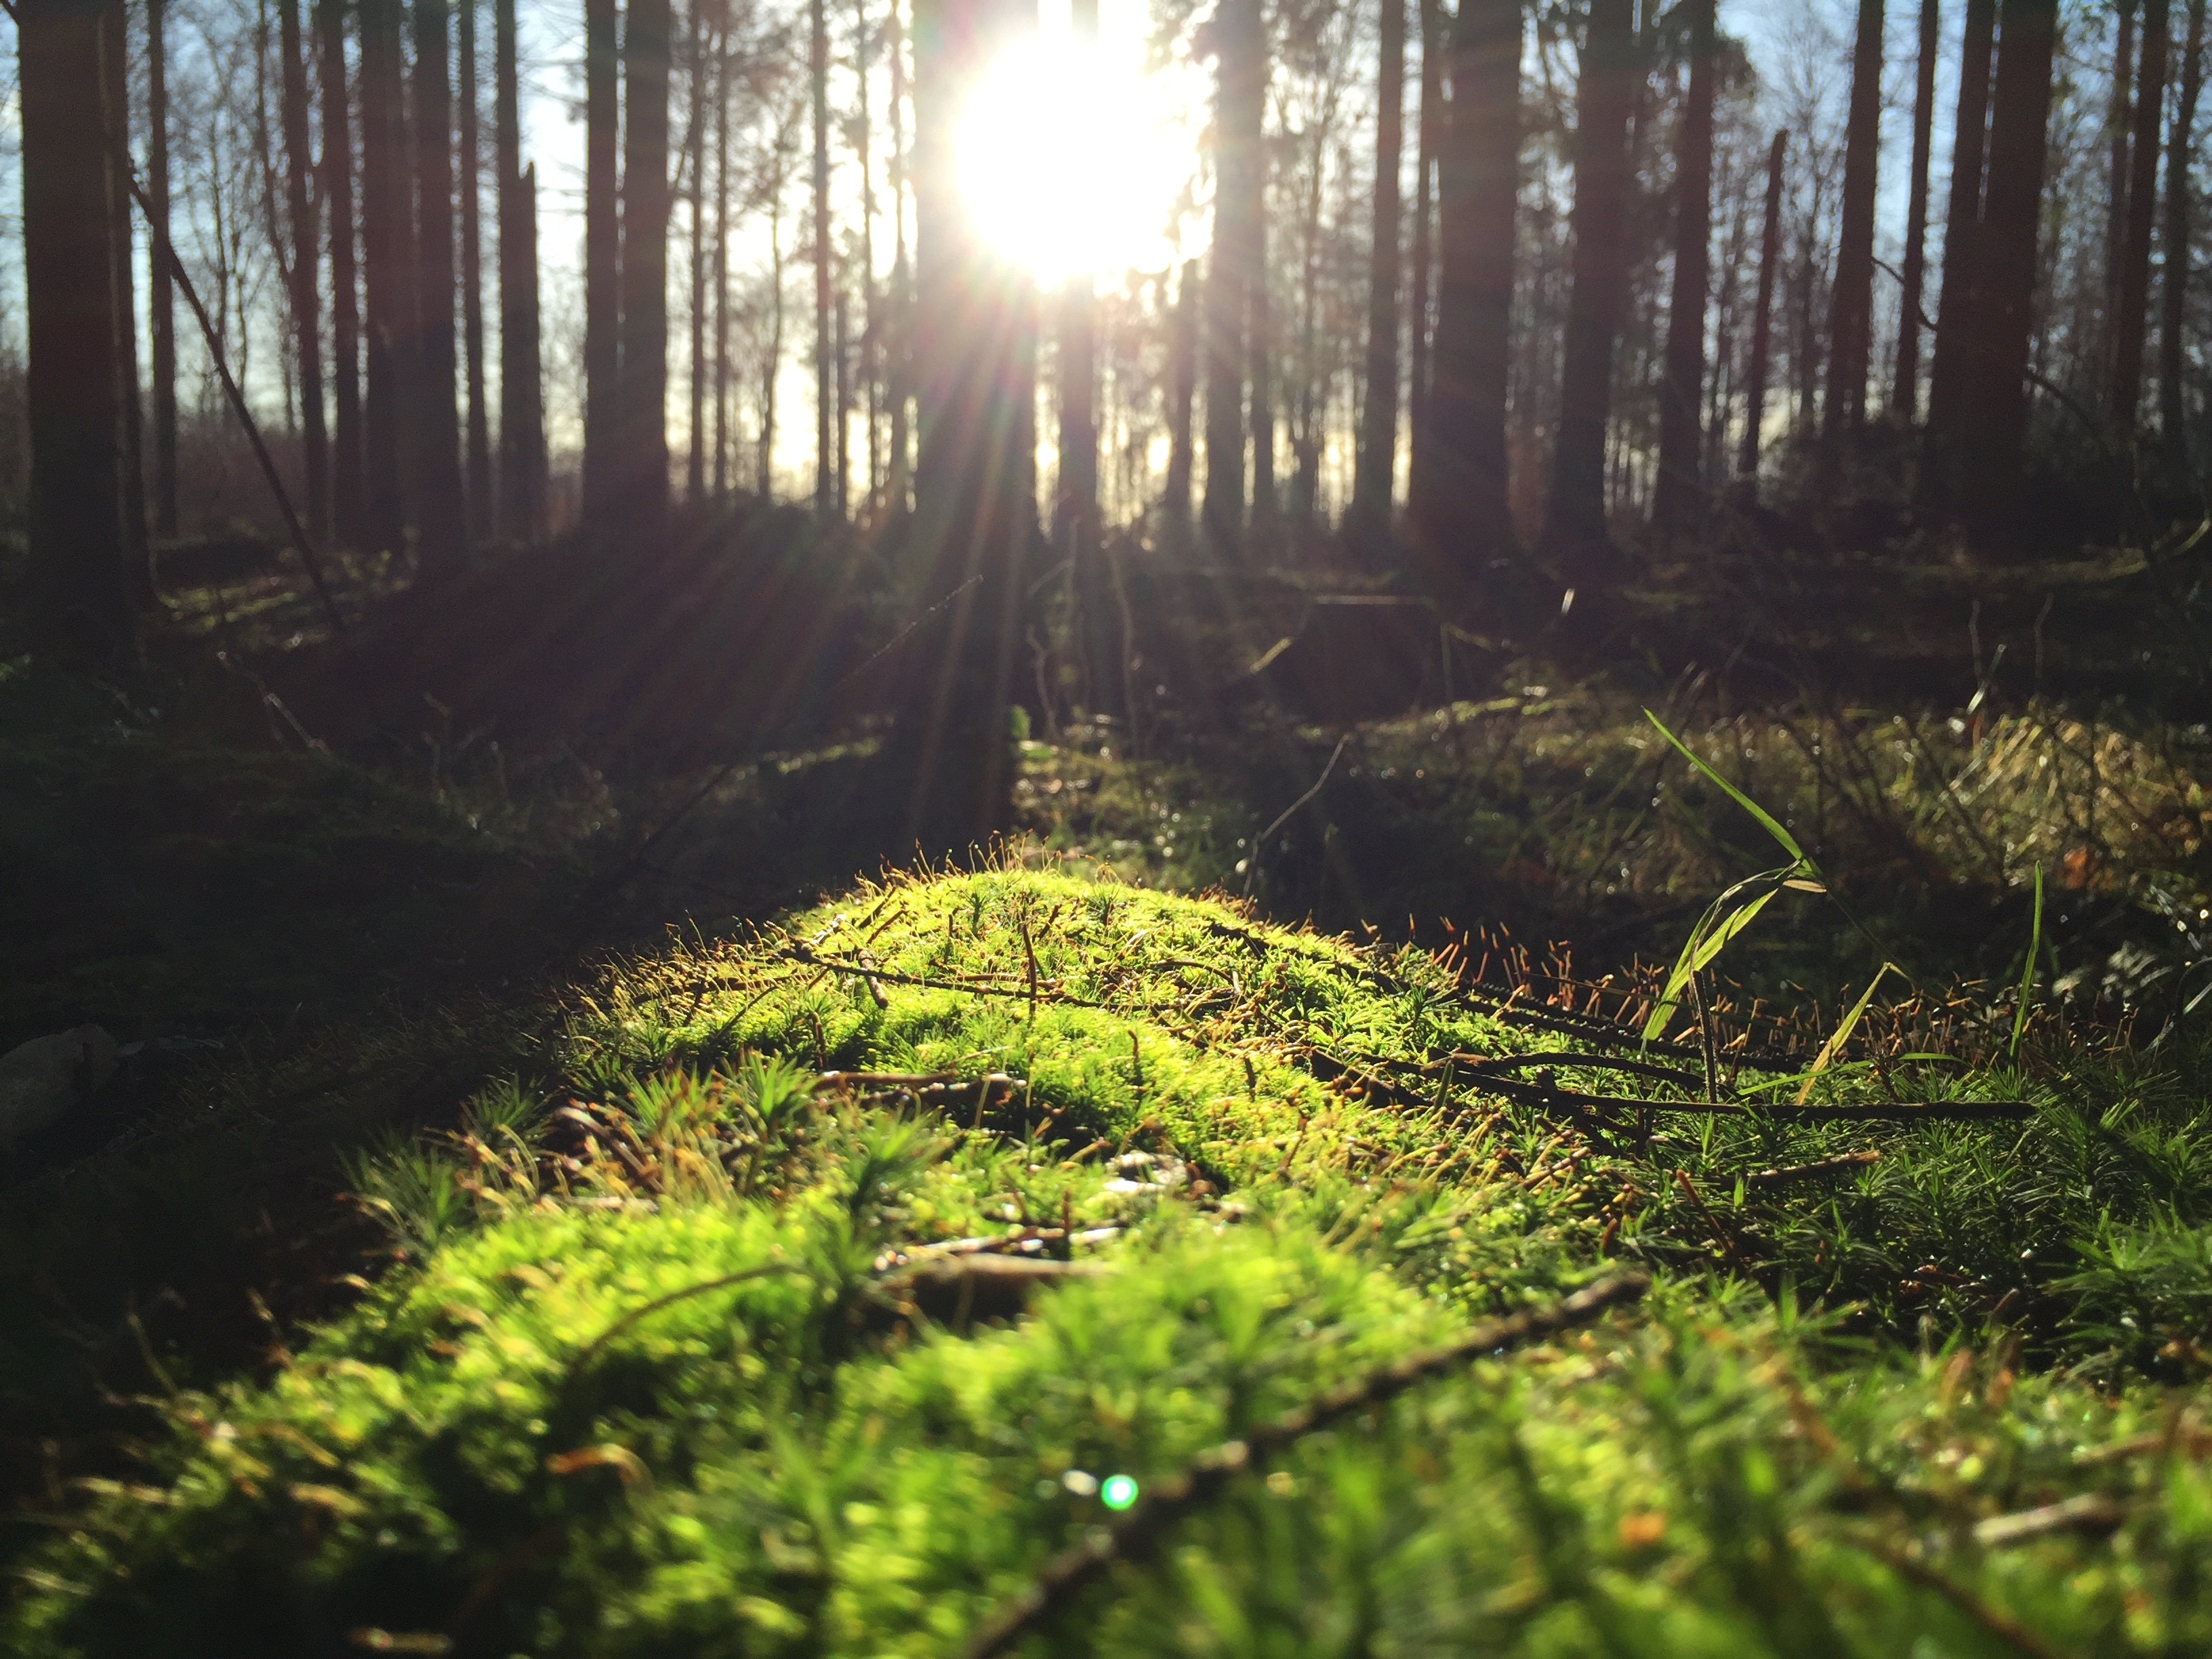
\includegraphics[width=1\linewidth]{figures/sunlight} 

}

\caption{Sunlight}\label{fig:sunlight}
\end{figure}

\textbf{\href{https://github.com/YoungjunNa/2019-animal-nutrition-and-the-environment/raw/master/03\%E1\%84\%8C\%E1\%85\%AE\%E1\%84\%8E\%E1\%85\%A1-\%E1\%84\%83\%E1\%85\%A9\%E1\%86\%BC\%E1\%84\%86\%E1\%85\%AE\%E1\%86\%AF\%E1\%84\%92\%E1\%85\%AA\%E1\%86\%AB\%E1\%84\%80\%E1\%85\%A7\%E1\%86\%BC\%E1\%84\%92\%E1\%85\%A1\%E1\%86\%A8.pdf}{강의자료
다운로드: 유전, 영양, 환경}}

\textbf{\href{https://youngjunna.github.io/aes/04-Light}{강의자료 보기:
Light}}

\section{Sunlight}\label{sunlight}

The main source of light on th earth is the sun. Sunlight provides the
energy that green plants use to create sugars mostly in the form of
starches, which release energy into the living things that digest them.
This process of photosynthesis provides virtually all the energy used by
living things. Some species of animals generate their own light, a
process called bioluminescence. For example, fireflies use light to
locate mates, and vampire squids use it to hide themselves from prey.

Daylight is the combination of all direct and indirect sunlight during
the daytime. Daytime is the period of time each day when daylight
occurs. \textbf{Daylight happens as the earth rotates, and either side
on which the sun shines is considered daylight.} Illuminance is a
measure of how much luminous flux is spread over a given area. The lux
(symbol: lx) is the SI derived unit of illuminance.

\begin{table}[t]

\caption{\label{tab:intensity}Light intensity in different conditions.}
\centering
\begin{tabular}{ll}
\toprule
Illuminance & Example\\
\midrule
120,000 lux & Brightest sunlight\\
111,000 lux & Bright sunlight\\
20,000 lux & Shade illuminated by entire clear blue sky, midday\\
1,000-2,000 lux & Typical overcast day, midday\\
400 lux & Sunrise or sunset on a clear day\\
\addlinespace
0.25 lux & A full Moon, clear night sky\\
0.01 lux & A quarter Moon, clear night sky\\
\bottomrule
\end{tabular}
\end{table}

\section{Photoperiodic response}\label{photoperiodic-response}

Photoperiodic response is the physiological reaction of organisms to the
length of day or night. A number of biological and behavioural changes
are dependent on the daylength. Together with temperature changes,
photoperiod provokes changes in the color of fur and feathers,
migration, entry into hibernation, sexual behaviour, and even the
resizing of sexual organs.

In animals, the regular activities of migration, reproduction, and the
changing of coats or plumage can be induced out of season by
artificially altering daylight. Long periods of light followed by short
periods will induce mating behaviour in species that normally breed in
autumn (e.g.~goats and sheep), while spring breeders (e.g.~mink) will
start the reproductive process when daylight is increased. Application
of photoperiodism is common in the poultry industry, as daylight affects
egg-laying, mating, and body weight of the fowl.

\section{Seasonal breeding}\label{seasonal-breeding}

\begin{figure}

{\centering 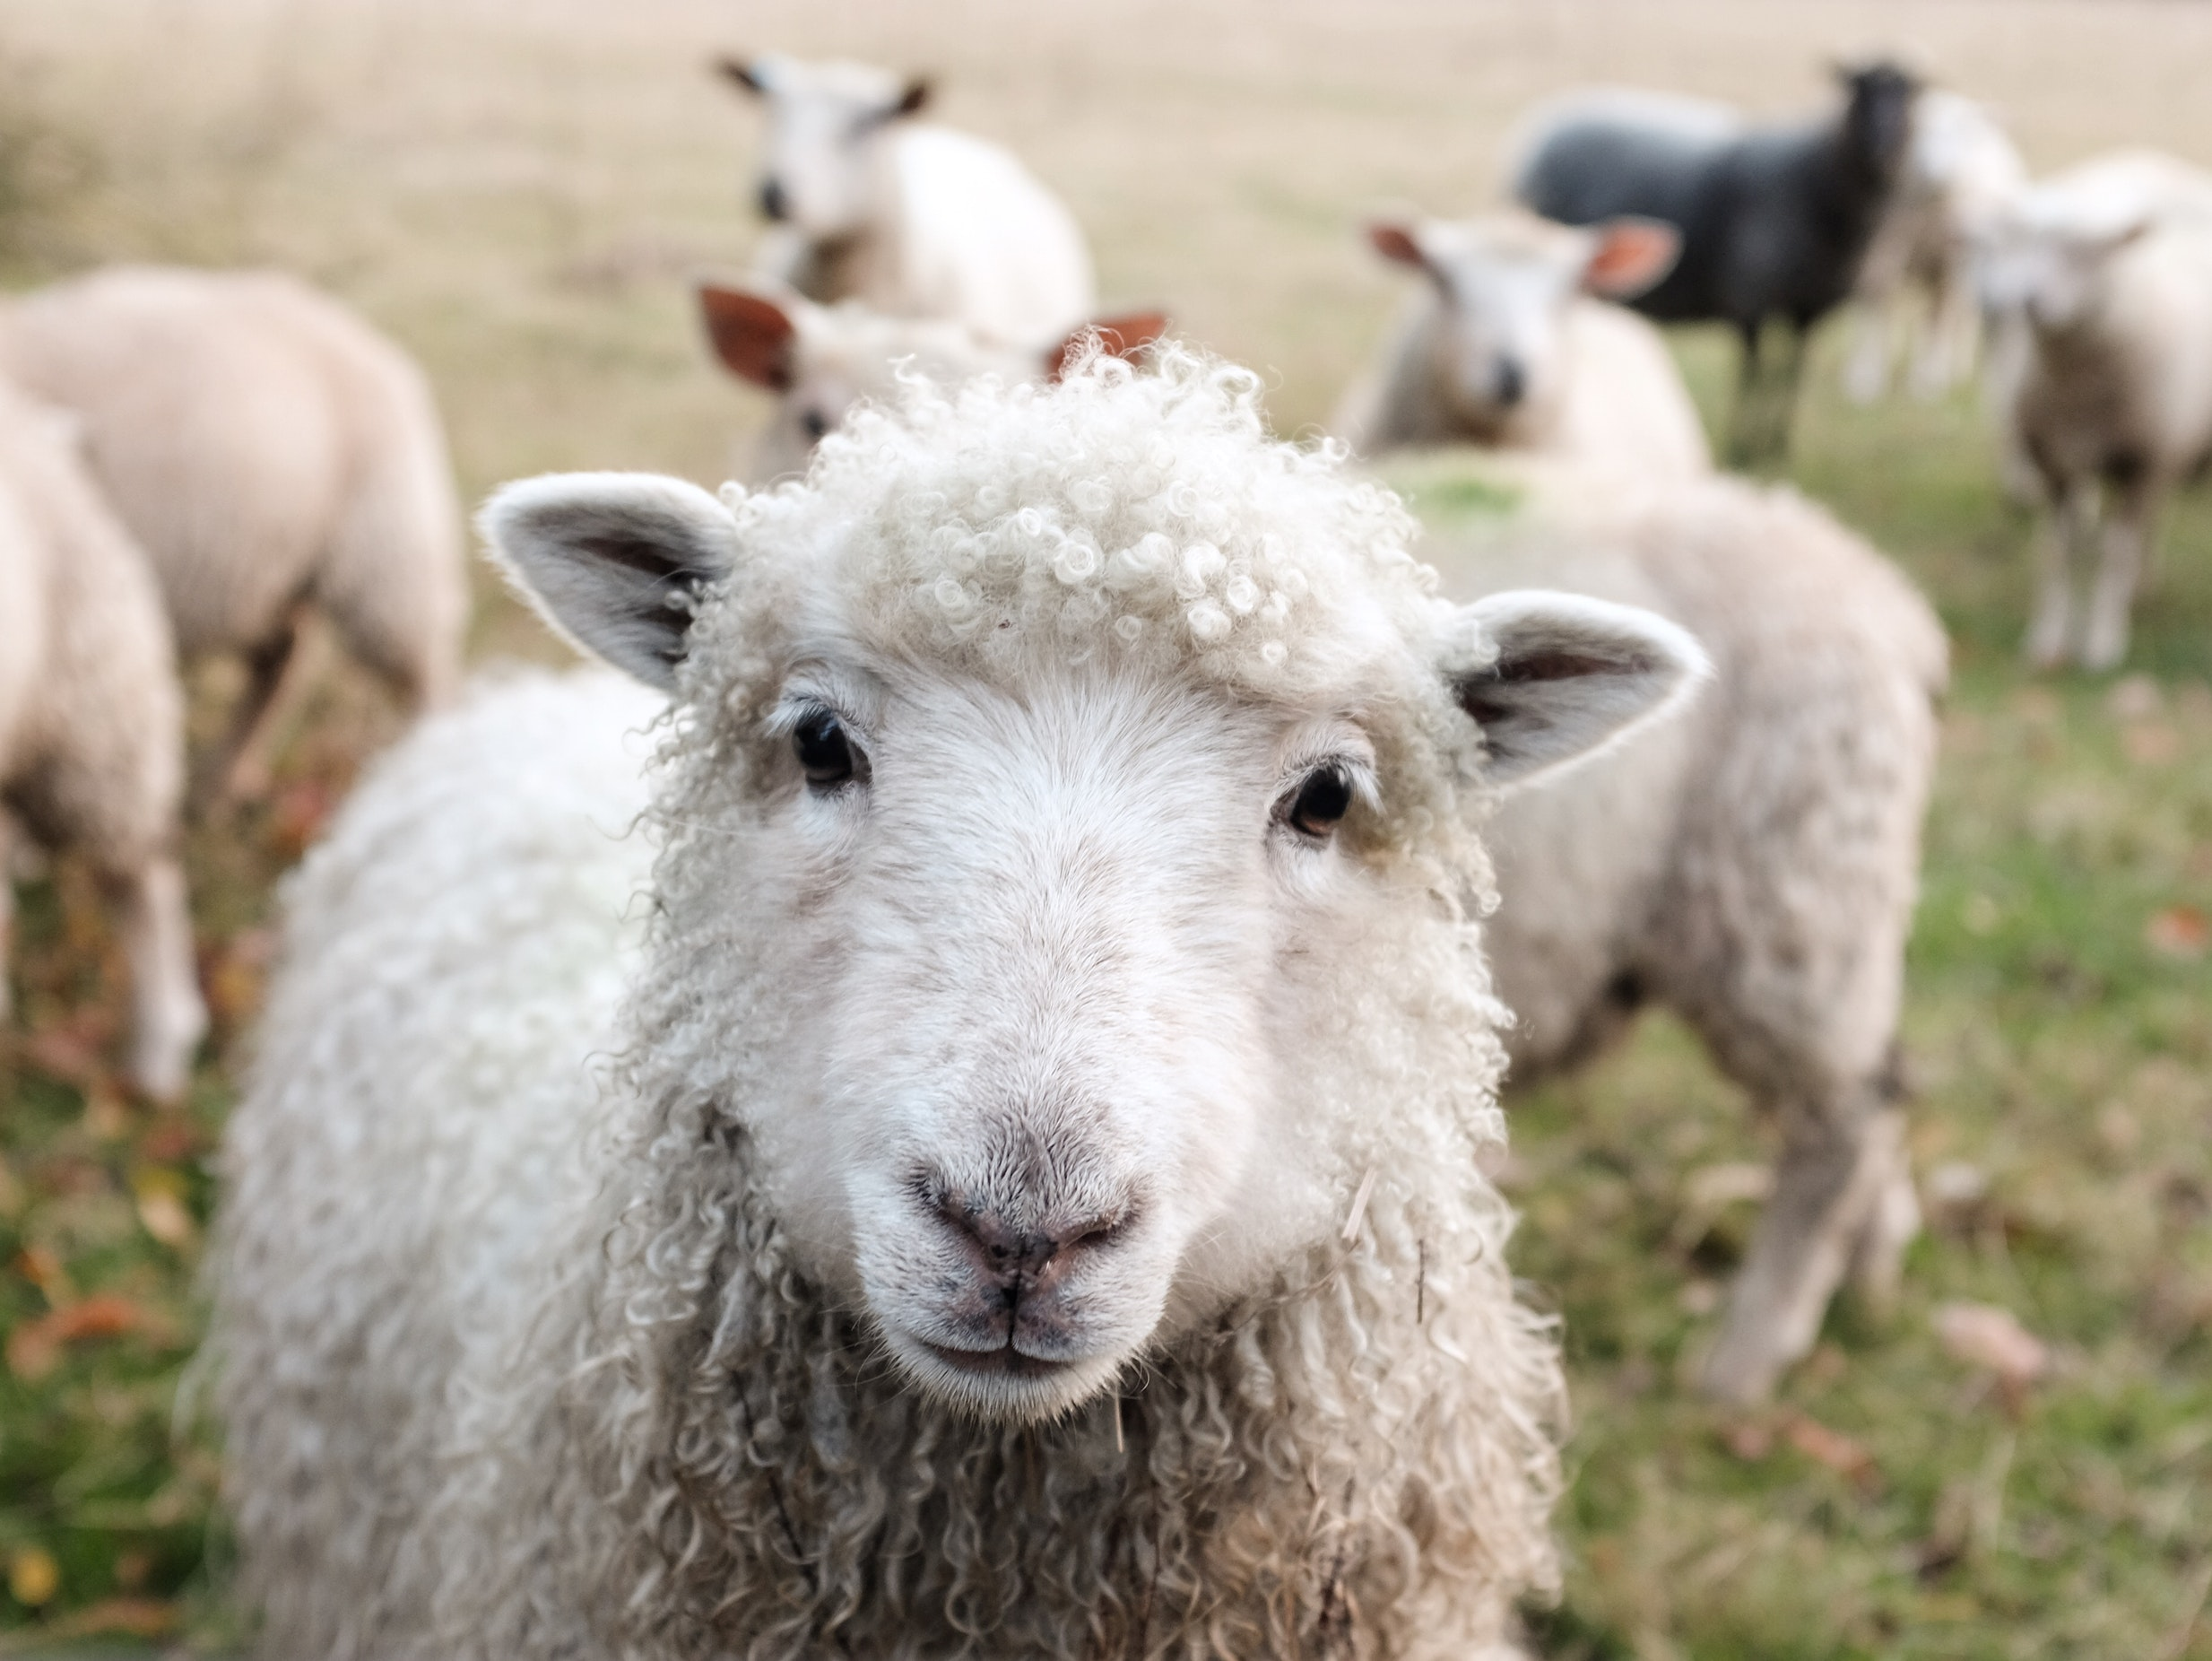
\includegraphics[width=1\linewidth]{figures/sheep} 

}

\caption{Sheep breeds when the length of daylight shortens}\label{fig:sheep}
\end{figure}

Seasonal breeders are animal species that successfully mate only during
certain times of the year. \textbf{These times of year allow for the
optimization of survival of young} due to factors such as ambient
temperature, food and water availability, and changes in the predation
behaviors of other species. Related sexual interest and behaviors are
expressed and accepted only during this period. Female seasonal breeders
will have one or more estrus cycles only when she is ``in season'' or
fertile and receptive to mating. Male seasonal breeders may exhibit
changes in testosterone levels, testes weight, and fertility depending
on the time of year.

The hypothalamus is considered to be the central control for
reproduction due to its role in hormone regulation. This is achieved
specifically through changes in the production of the hormone GnRH. GnRH
in turn transits to the pituitary where it promotes the secretion of the
gonadotropins LH and FSH, both pituitary hormones critical for
reproductive function and behavior, into the bloodstream.

\begin{figure}

{\centering 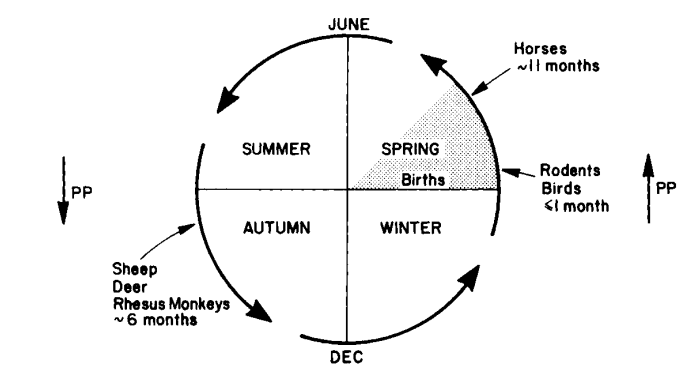
\includegraphics[width=0.7\linewidth]{figures/seasonal-breed} 

}

\caption{Timing of annual reproductive cycle of exemplary seasonal breeders. PP, photoperiod. }\label{fig:seaonal-breed}
\end{figure}

Seasonal breeding readiness is strongly regulated by length of day
(photoperiod) and thus season. Photoperiod likely affects the seasonal
breeder through changes in melatonin secretion by the pineal gland that
ultimately alter GnRH release by the hypothalamus. Seasonal breeders can
be divided into groups based on fertility period. \textbf{``Long day''}
breeders (horse, hamsters, and mink) cycle when days get longer (spring)
and are in anestrus in fall and winter. \textbf{``Short day''} breeders
(sheep, goat, and elk) cycle when the length of daylight shortens (fall)
and are in anestrus in spring and summer.

\subsection{Antlers}\label{antlers}

\begin{figure}

{\centering 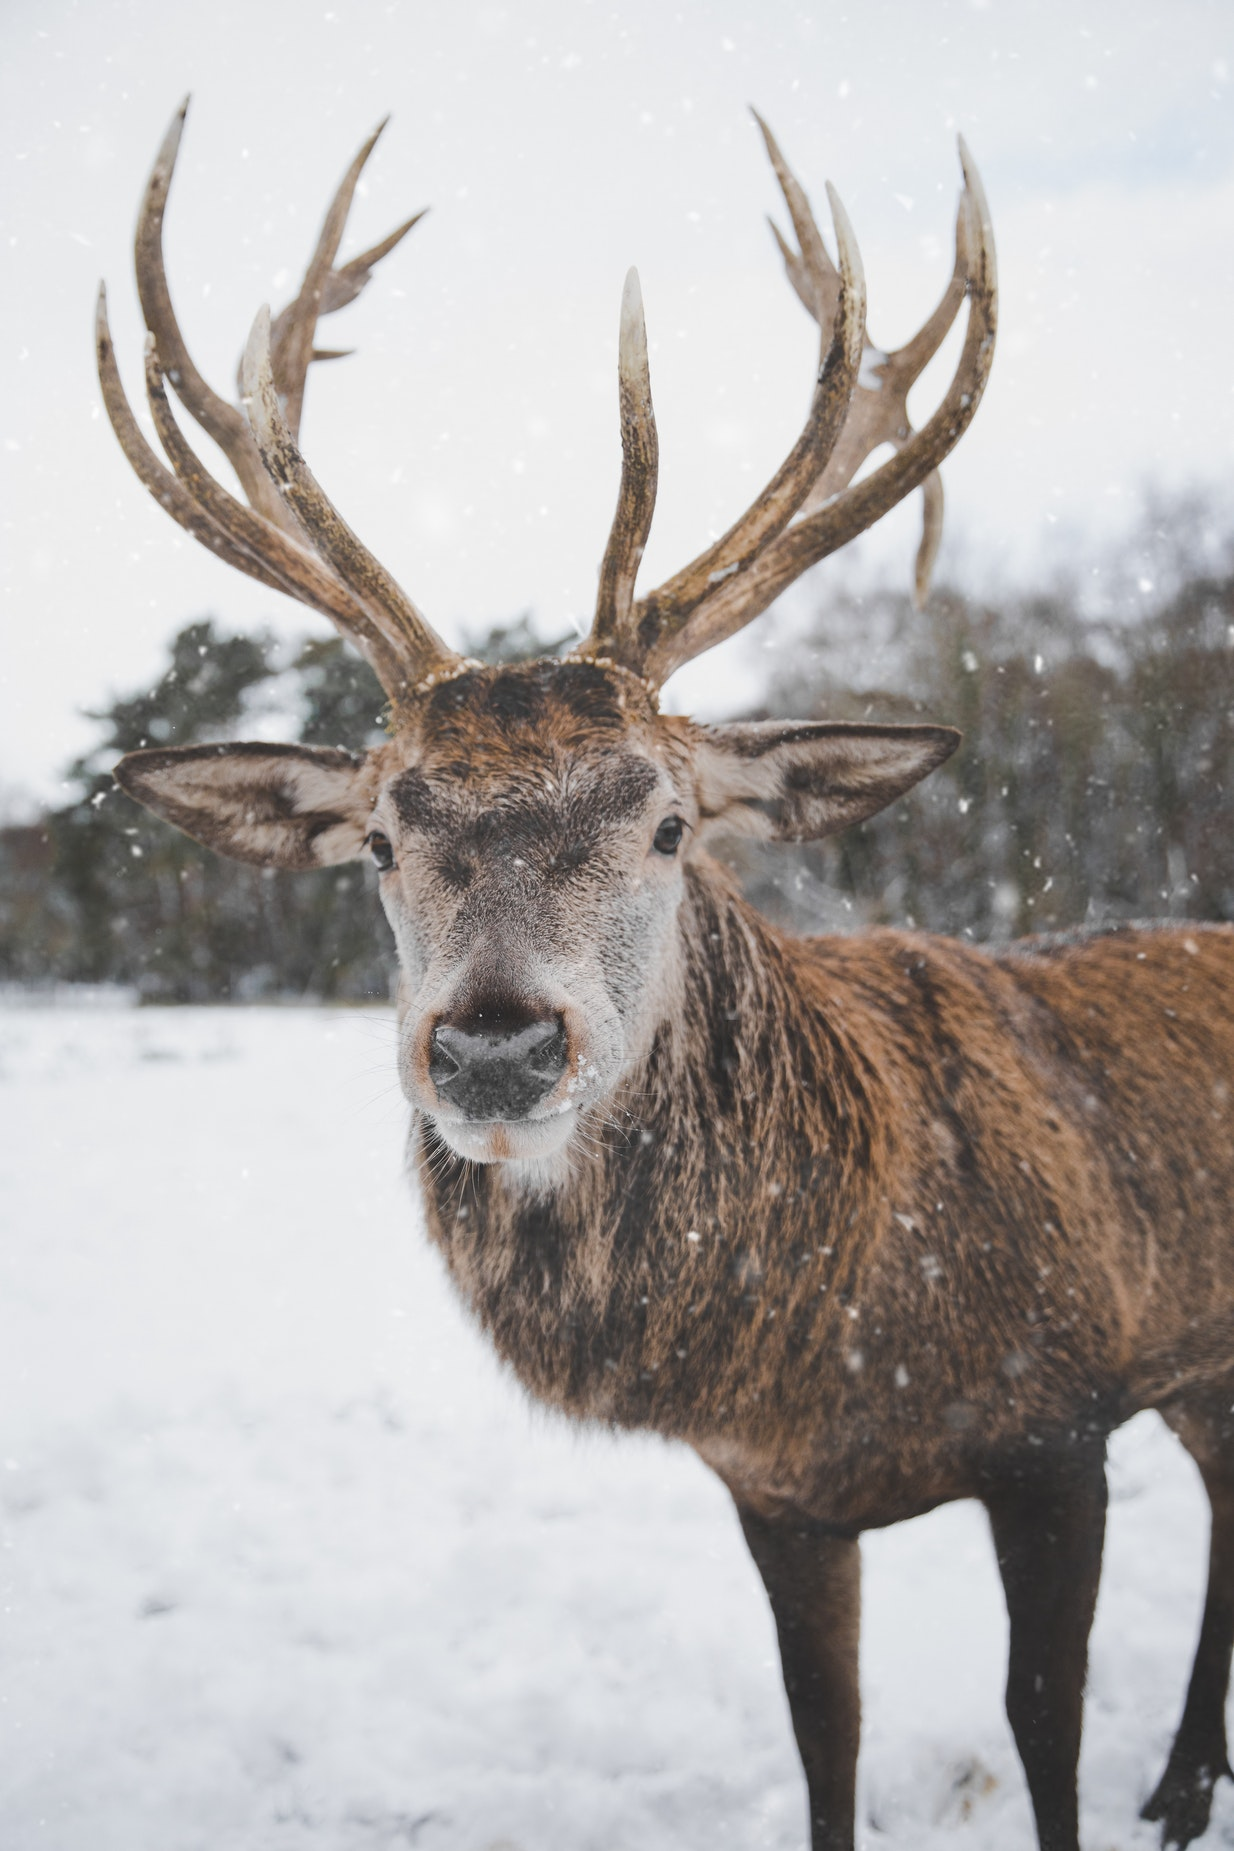
\includegraphics[width=0.6\linewidth]{figures/antler} 

}

\caption{Antlers are shed and regrown each year.}\label{fig:antler}
\end{figure}

Antlers are extensions of an animal's skull found in members of the deer
family. Antlers are shed and regrown each year (grown every spring and
shed every winter) and function primarily as objects of sexual
attraction and as weapons in fights between males.

\textbf{The annual antler cycle is ultimately controlled by day length
or photoperiod.} Growth of antlers typically begins in April in response
to increasing day length. In the spring, testicular and pituitary
hormones get the growing process started. Antlers are covered with
velvet (such as in the antlers of the deer in the photo above) which
carries blood and nutrients to the antlers during development. By late
summer, as day length decreases, testosterone levels begin to increase,
the form is filled, and the antler begins to harden. Hard antlers remain
on the deer through the peak of breeding until late fall or early
winter. In winter, when the growth hormones quit pumping, the pedicel
loses calcium which weakens the connection between the pedicel and the
antler, and off come the antlers.

\begin{figure}

{\centering 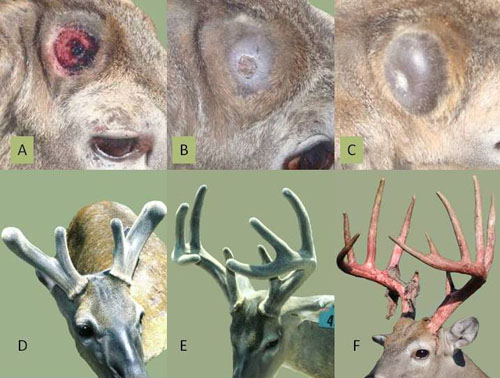
\includegraphics[width=1\linewidth]{figures/antler-stages} 

}

\caption{Stages of antler growth. A) one day after antler shed, B) 15 days after shed, scab still attached, C) 30 days after shed, scab is shed (A, B, C same animal), D) about three months after shed by different animal, E) about five months after shed antler growth is completed, with one additional month used to complete hardening and drying of velvet (D and E same animal), and F) hardened antler with shreds of dried velvet on a third animal. (Photo Credits A-E, Steve Demarais, F, Dave Hewitt)}\label{fig:antler-stage}
\end{figure}

Horns, on the other hand, are found on members of the \emph{Bovidae}
family, which includes species as diverse as cows, sheep and goats to
water buffalo, antelopes, and gazelles. Unlike antlers, horns are never
branched, are never shed, and in many species horns never stop growing
throughout an animal's life.

\section{Effects on productivity}\label{effects-on-productivity}

\subsection{Light control in poultry
production}\label{light-control-in-poultry-production}

Lighting is a key environmental factor in poultry production that is
known to affect performance and behavior. The photoperiod is the
duration of the light period and scotoperiod is the duration of the dark
period perceived in a light:dark cycle, which is typically 24 h in
length.

\subsubsection{Broiler}\label{broiler}

Modern broiler stocks have been genetically selected for rapid growth,
heavy BW, feed efficiency, and high breast meat yield. The inactive
nature of fully-fed broilers in combination with early attainment of
heavy BW has contributed to developmental leg abnormalities. Lighting
programs have been developed based on their effectiveness in the
industry to optimize performance. The performance parameters of broilers
in which producers are most interested are BW, feed efficiency, and
livability. \textbf{Continuous lighting (24L:0D) leads to greater BW for
meat-type chickens compared to those under 8L:16D or 12L:12D.}
Generally, longer dark period leads to greater feed efficiency.

\begin{table}[t]

\caption{\label{tab:lightening}An example of broiler lighting program.}
\centering
\begin{tabular}{lrrr}
\toprule
Days & Light (h) & Dark (h) & Intensity (lux)\\
\midrule
0 & 23 & 1 & 20\\
1-2 & 20 & 4 & 20\\
3-4 & 18 & 6 & 20\\
5-14 & 6 & 18 & 5\\
15-21 & 10 & 14 & 5\\
\addlinespace
22-28 & 14 & 10 & 5\\
29-35 & 18 & 6 & 5\\
36-42 & 24 & 0 & 5\\
\bottomrule
\end{tabular}
\end{table}

\subsubsection{Layers}\label{layers}

Layer hens require a minimum amount of light intensity for optimal egg
production, usually 5 to 10 lux. Both estrogen and progesterone are
required to form eggs, and a short daylength will not stimulate the
secretion of these hormones.

\textbf{The color of light has been shown to affect the size and weight
of the eggs.} Blue-green light stimulates growth in chickens, whereas
orange-red light stimulates reproduction. Red light, in the 630nm
wavelength range, was found to be superior to any other wavelength in
increasing egg production. However, blue light has a calming effect on
birds whereas red may enhance feather pecking and cannibalism.

\section{Appendix}\label{appendix}

\chapter{Sound}\label{sound}

\begin{figure}

{\centering 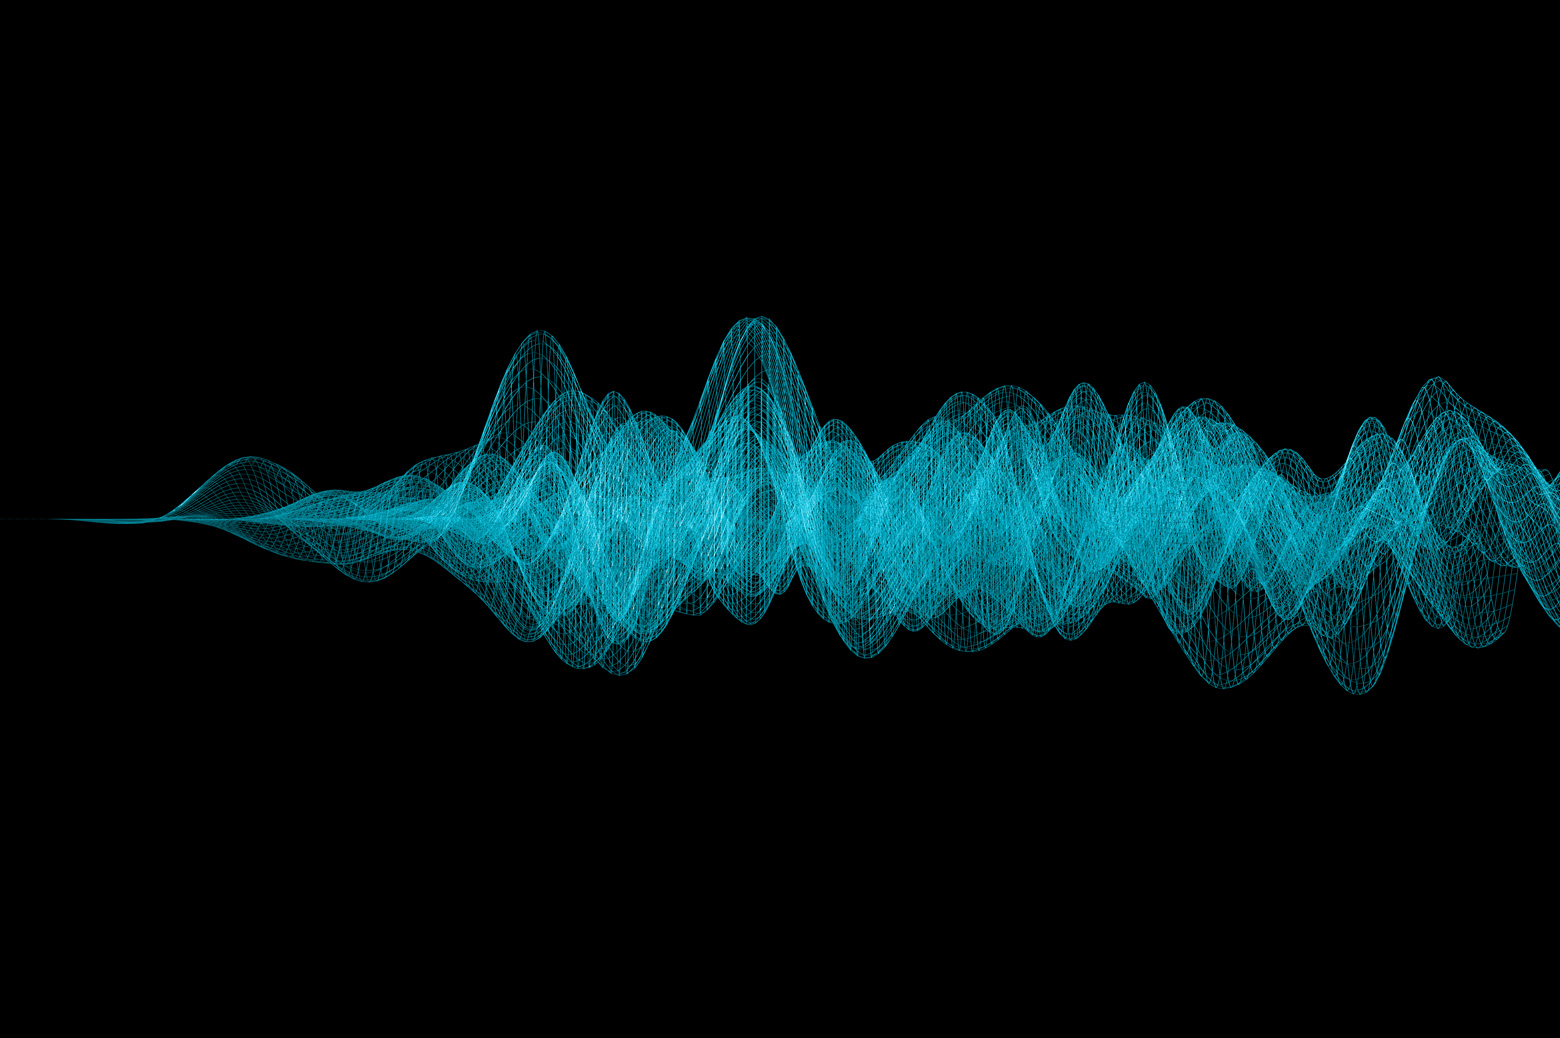
\includegraphics[width=1\linewidth,height=0.5\textheight]{figures/soundwave} 

}

\caption{Sound is a vibration that typically propagates as an audible wave of pressure.}\label{fig:soundwave}
\end{figure}

\textbf{\href{https://github.com/YoungjunNa/aes/raw/master/04-aes.pdf}{강의자료
다운로드: 인간, 동물, 환경}}

\textbf{\href{https://youngjunna.github.io/aes/05-Sound}{강의자료 보기:
Sound}}

\begin{quote}
``One good thing about music, when it hits you, you feel no pain.'' ---
Bob Marley
\end{quote}

\textbf{Sound is a vibration that typically propagates as an audible
wave of pressure, through a transmission medium such as a gas, liquid or
solid.} The sound waves are generated by a sound source, such as the
vibrating diaphragm of a stereo speaker. The sound source creates
vibrations in the surrounding medium. The speed of sound is the distance
travelled per unit time by a sound wave as it propagates through an
elastic medium. At 20 °C, the speed of sound in air is about 343 m/s.

The hertz (Hz) is the derived unit of frequency in the SI and is defined
as one cycle per second. A decibel (dB) measures ratios of power or
intensity. The decibel is not an SI unit.

\begin{table}[t]

\caption{\label{tab:db}Examples of different level of decibel.}
\centering
\begin{tabular}{ll}
\toprule
Sound Level & Examples\\
\midrule
171 dB & Next to a loud rifle being shot\\
150 dB & Right next to a jet engine\\
110-140 dB & Jet engine at 100 meters\\
130-140 dB & Where most people begin to feel pain\\
130 dB & Trumpet (a half meter in front of)\\
\addlinespace
120 dB & Vuvuzela horn (1 meter in front of), risk of immediate hearing loss\\
110 dB & Gas chainsaw\\
100 dB & Jack hammer\\
80-90 dB & Traffic on a busy roadway\\
60-80 dB & Passenger car\\
\addlinespace
40-60 dB & Normal conversation\\
20-30 dB & Very calm room\\
10 dB & Light leaf rustling, calm breathing\\
0 dB & Hearing threshold right next to ear\\
\bottomrule
\end{tabular}
\end{table}

\section{Perception of sound}\label{perception-of-sound}

The physical reception of sound in any hearing organism is limited to a
range of frequencies. Humans normally hear sound frequencies between
approximately 20 Hz and 20,000 Hz (20 kHz). The upper limit of sound
frequency decreases with age. Dogs can perceive vibrations higher than
20 kHz. Ultrasound is sound waves with frequencies higher than 20,000
Hz. Infrasound is sound waves with frequencies lower than 20 Hz.
Although sounds of such low frequency are too low for humans to hear,
whales, elephants and other animals can detect infrasound and use it to
communicate.

\textbf{Sound is used by many species for detecting danger, navigation,
predation, and communication.} Earth's atmosphere, water, and virtually
any physical phenomenon, such as fire, rain, wind, surf, or earthquake,
produces its unique sounds. Many species, such as frogs, birds, marine
and terrestrial mammals, have also developed special organs to produce
sound. In some species, these produce song and speech. Furthermore,
humans have developed culture and technology (such as music, telephone
and radio) that allows them to generate, record, transmit, and broadcast
sound.

\section{Vocalization}\label{vocalization}

Animal vocalization refers to any sound an animal may make to
communicate a message to others. All birds and mammals are able to
vocalize. They use the voice as communication signals to indicate some
types of ``need''.

With increasing interest in measures of welfare ``from the animal's
point of view'' the study of vocalizations of the animal is still in the
focus of interest. The vocalization of pigs has been a topic of research
since nearly half a century. The vocalization in pigs is strongly
related to their level of excitement. Low-pitched vocalizations with low
tonality such as grunts are used to maintain social contact with group
mates. Louder and longer but high-pitched calls such as screams are more
related to the state of excitement. Xin et al. (1989) demonstrated that
in a production environment several types of pig vocalizations can be
distinguished.

\begin{center}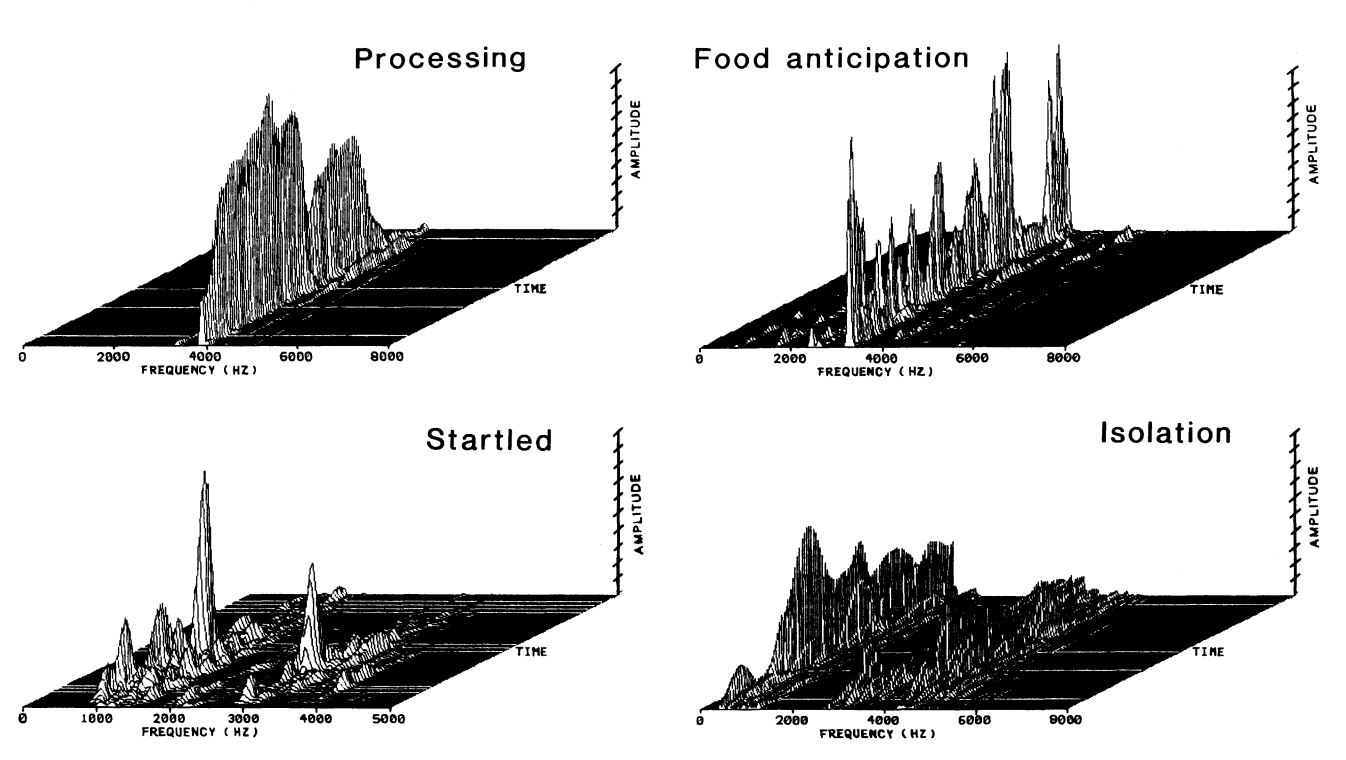
\includegraphics[width=1\linewidth]{figures/pig-vocal1} \end{center}

\begin{figure}

{\centering 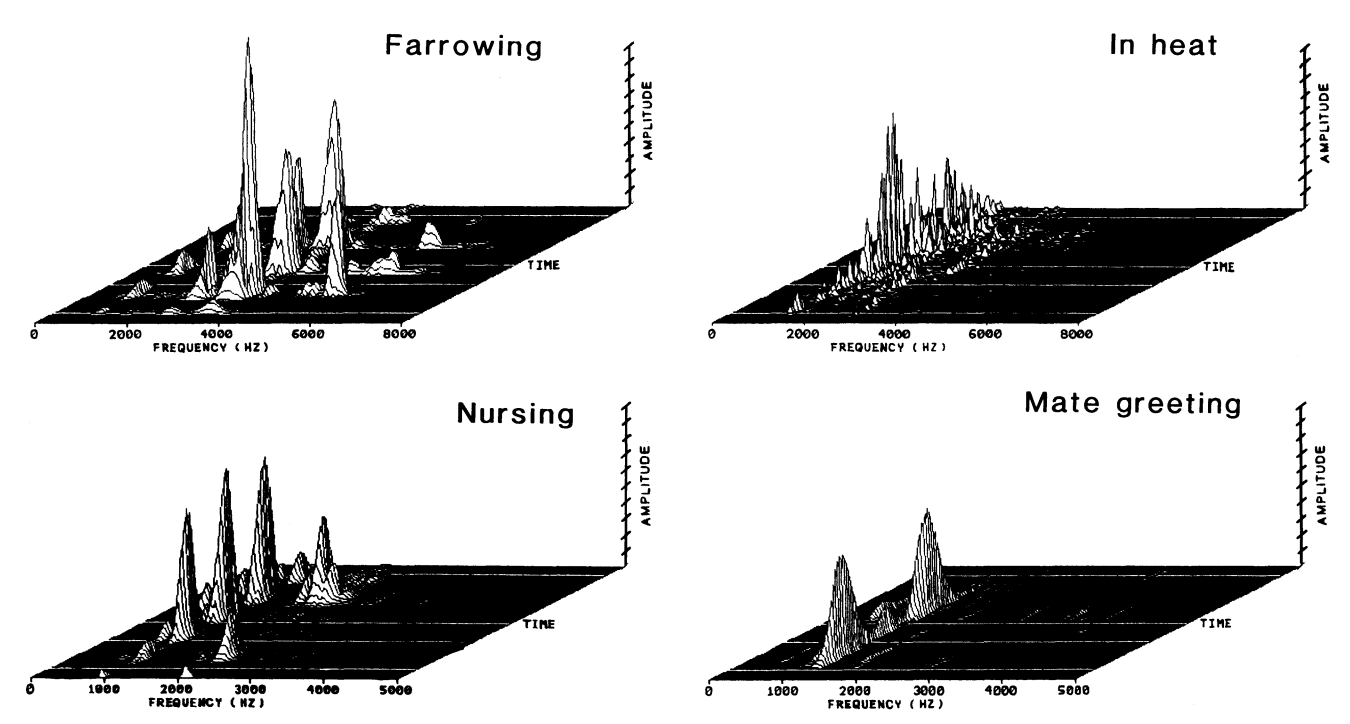
\includegraphics[width=1\linewidth]{figures/pig-vocal2} 

}

\caption{Sonographs of pig vocalizations (Xin et al., 1989).}\label{fig:pig-vocalization}
\end{figure}

A great number (roughly 30) of different vocalizations have been
described for adult and juvenile chickens (Collias and Joos, 1953,
Baumer, 1962, Guhl, 1968, Wood-Gush, 1971, Huber and Folsch, 1978,
Wennrich, 1981).

\section{Noise and animal stress}\label{noise-and-animal-stress}

Noise is described as unwanted sound, either chronic or intermittent,
and can be described in terms including its frequency, intensity,
frequency spectrum, and shape of sound pressure through time (Burn,
2008). Decibel (dB) is the unit for measuring the intensity of sound.

Noise in farm animal environments is a detrimental factor to animal
health. Noise directly affects reproductive physiology or energy
consumption. Unexpected high intensity noise (above 110 dB), such as low
altitude jet aircraft overflights at milking time could reduce the
overall milk yield. However, a majority of the studies reviewed suggests
that there is little or no effect of aircraft noise on cattle. Beyer
(1983) found that helicopters caused worse reaction than other
low-aircraft overflights.

Sounds produced by humans might also be stressful for farm animals. Loud
cry causes stress responses in farm animals (Hemsworth et al., 2003).
Shouting on dairy cows appears to be very aversive (Pajor et al., 2000).
Noise made by humans shouting and slamming of metal gates increases
heart rate and activity in cattle.

Although the majority of the literature suggests that farming animals
and wildlife species exhibit adaptation after repeated exposure to
noise, careful planning should be made before construction of the animal
building, in order to avoid stressful environmental sounds both for the
animal and personnel.

\section{Music and animal welfare}\label{music-and-animal-welfare}

Humans derive both psychological and physiological benefits from
listening to music, including reduced anxiety, pain relief and decreases
in measures of stress such as blood pressure and heart rate. Some
nonhuman species may perceive music similarly to humans, but because of
species differences in sensitivity to sound frequencies, music may be
perceived differently by different species. For example, most studies
examining the physiological effects of music to date used rats, but most
of the common laboratory rat's social communication occurs in the
ultrasonic range.

The type of music to which an animal is exposed is an important factor
in determining whether the music will have any effect on the animal.
Tempo, rhythm, pitch and tonality, may also influence the effects of
music on the physiology of animals. `New age' music has been reported to
have a `calming' effect on mice in comparison to classical or pop music
or the absence of music. Raising chicks with music enrichment can
decrease their stress levels. Music has been used to manipulate
physiology in order to improve milk production in dairy cattle and
growth of poultry, swine, and fish.

\begin{figure}

{\centering 
\includegraphics[width=1\linewidth]{figures/coldplay} 

}

\caption{A band make the sound.}\label{fig:coldplay}
\end{figure}

\section{Appendix}\label{appendix-1}

\chapter{Air quality}\label{air-quality}

\begin{figure}

{\centering 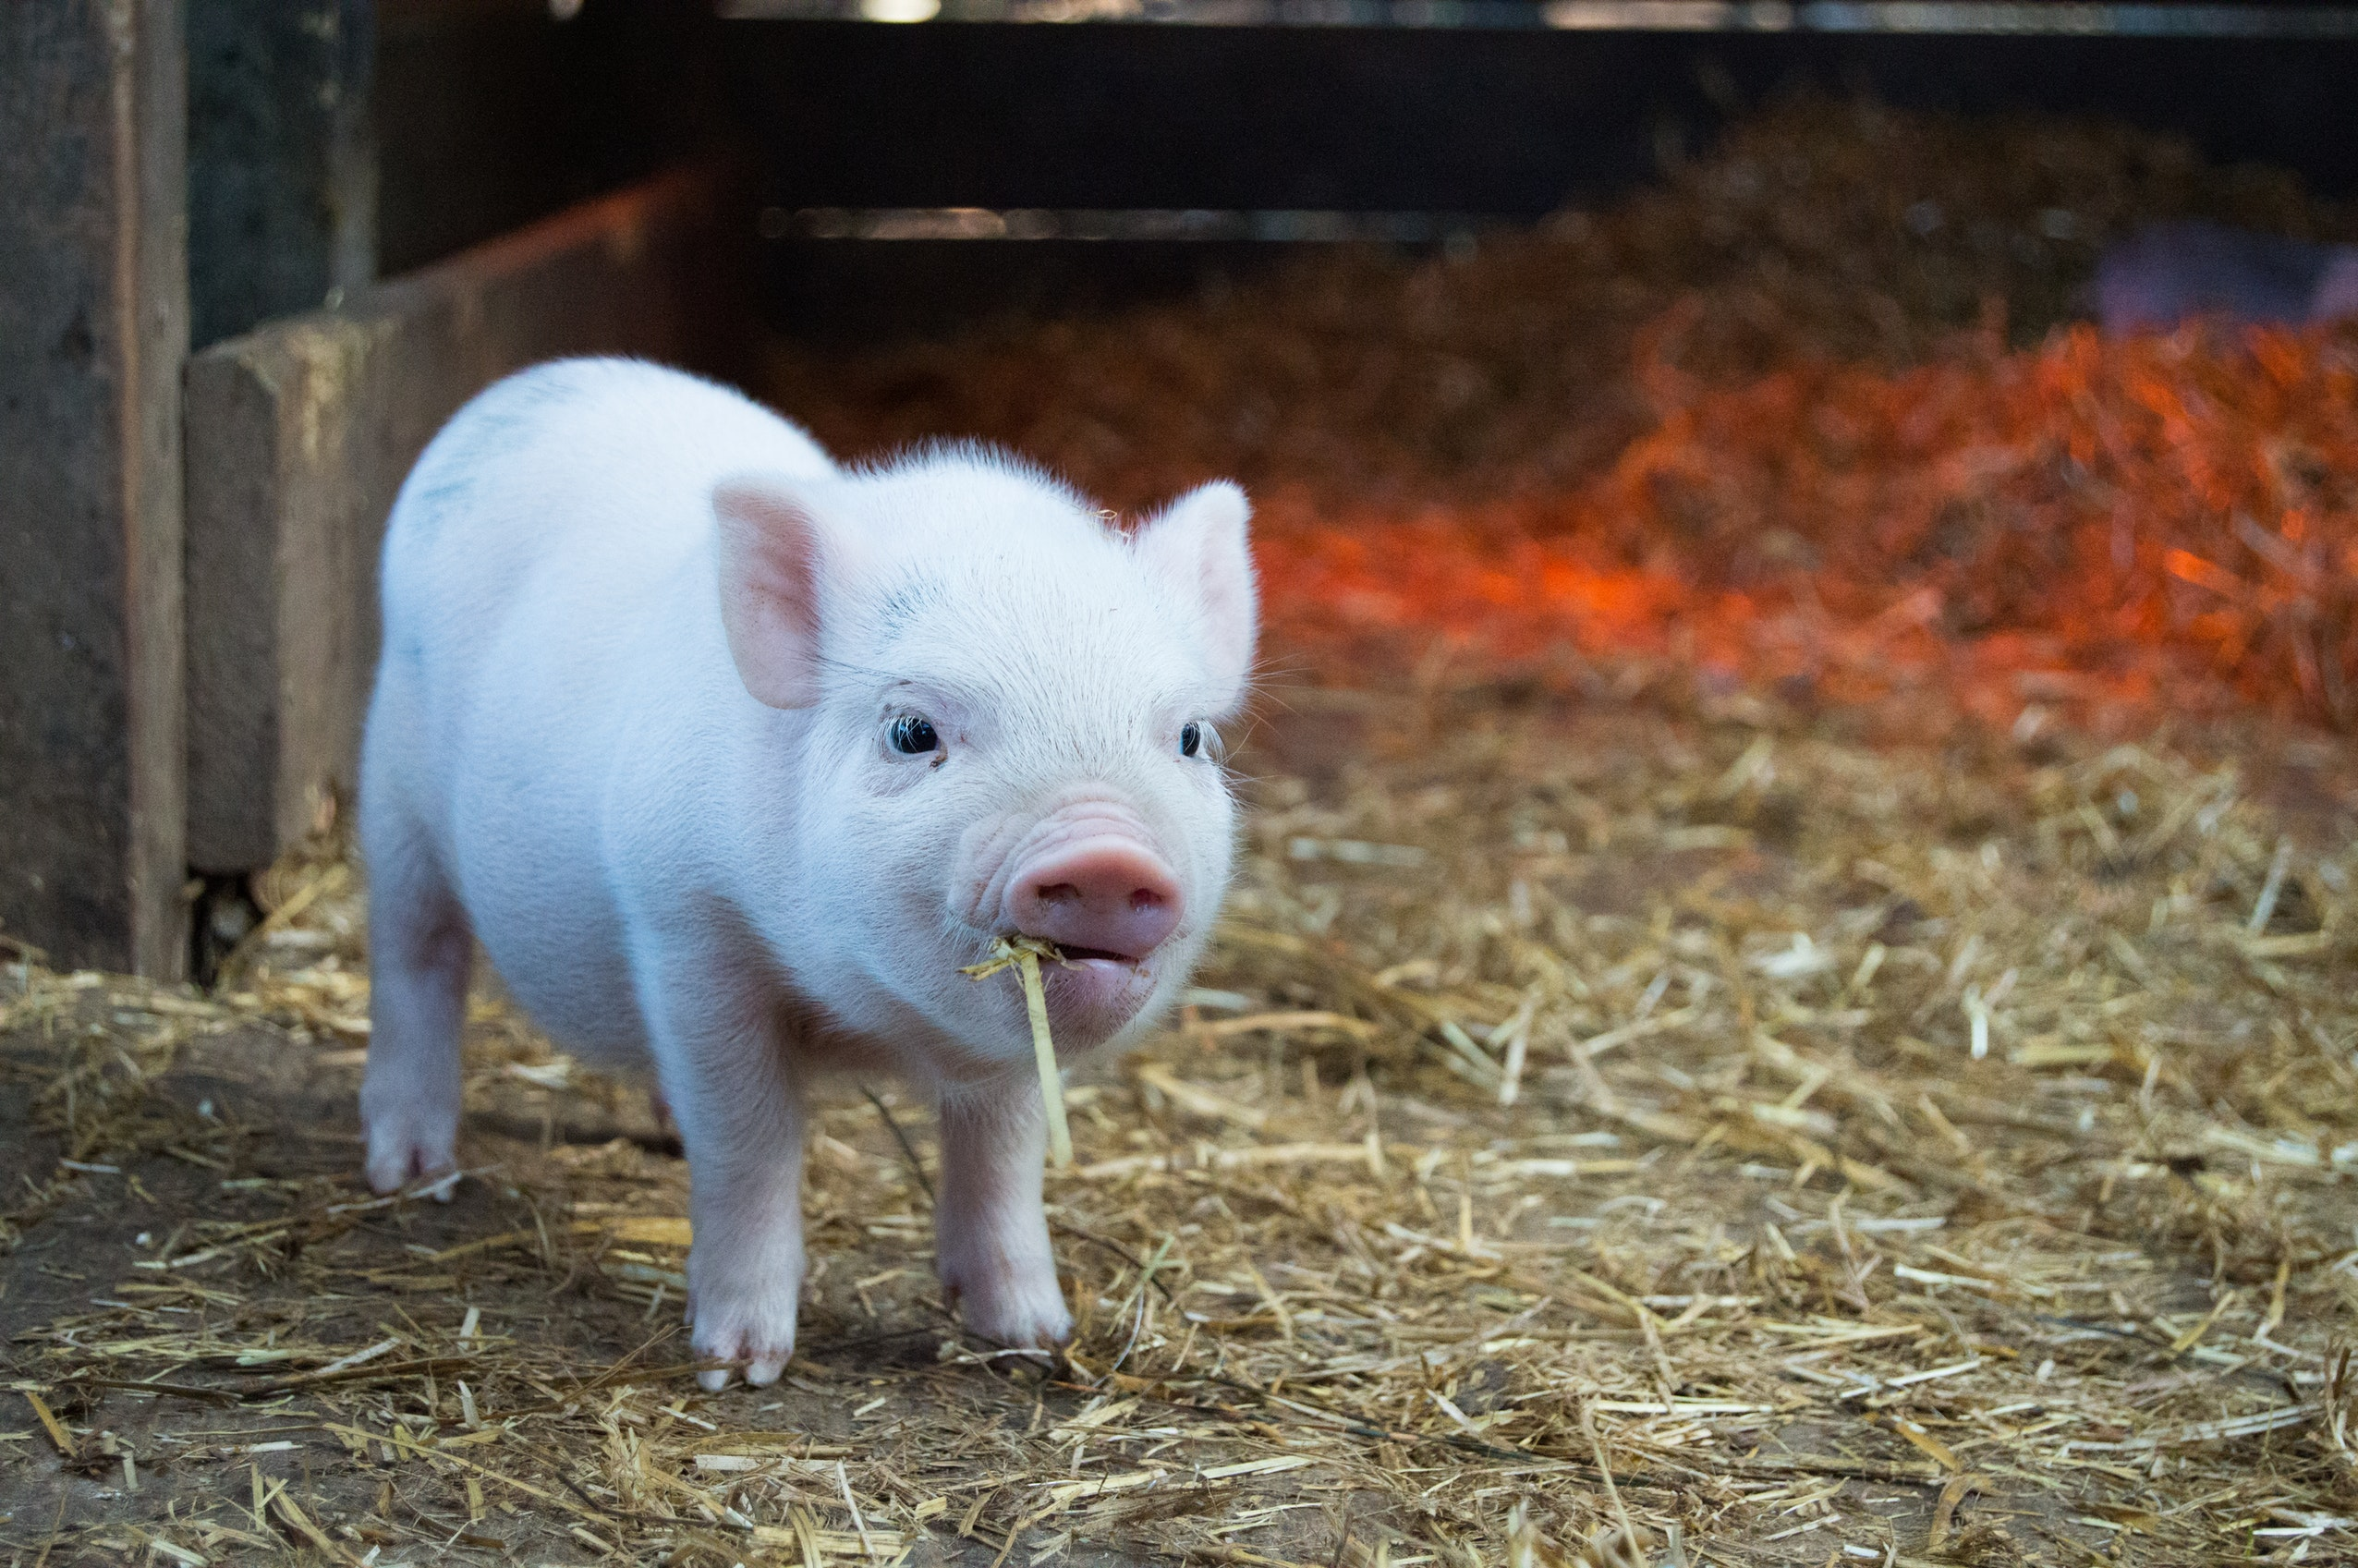
\includegraphics[width=1\linewidth,height=1\textheight]{figures/pig-straw} 

}

\caption{A white piglet chewing hay}\label{fig:pig-straw}
\end{figure}

\textbf{Air quality is the degree of pollution of air.} The air quality
can be determined by measuring the concentration of pollutants in the
air. Air quality has a direct influence on health, welfare and
production performance of livestock. The high concentrations of noxious
gases, dust, and airborne microorganisms can reduce the production
efficiency and the general welfare of farm animals. Long term exposure
to particulates in livestock buildings might also affect the respiratory
health of farm workers. Dust in animal buildings contains many
biologically active substances such as bacteria, fungi, and endotoxins
that are suspected to be hazardous to human health.

Airborne emissions include ammonia, methane, nitrous oxide, particulates
like dust and microorganisms. In addition, other potentially harmful
substances such as heavy metals, antibiotic residues and components of
disinfectants might be also emitted from livestock building that are
potentially damaging to ecosystems.

\section{Importance of air quality}\label{importance-of-air-quality}

Animals that continually exposed to bad air quality had reduced
productivity and increased the stress. Maintaining good air quality is
not only important for the productivity of the animals, but also for the
welfare of the animals.

\textbf{There are some benefits of improving the air quality:}\\
1. Improves the health, welfare and production performance of the
animals.\\
2. Improves the health and safety of producers and workers.\\
3. Reduces emissions of harmful pollutants to the outside environment
which helps reduce nuisance complaints.\\
4. Results in significant energy and economic savings.\\
5. Prolongs the life of building structures.

Generally air quality is affected by weather, livestock facilities and
management conditions. Air quality is getting worse during light wind
conditions, as pollutants cannot be blown away.

\section{Pollutants}\label{pollutants}

\subsection{Ammonia}\label{ammonia}

Ammonia (NH3) is an important pollutant gas that accelerates fine
particulate formation in the atmosphere and plays a crucial role in the
acidification and the eutrophication of ecosystems (Krupa, 2003).
Livestock wastes account for 39\% of global emissions (Fig.
\ref{fig:ammonia-manure}). Among them, pig production is globally
responsible for about 15\% of NH3 emissions associated to livestock,
with a large variation by country (Olivier et al., 1998).

\begin{figure}

{\centering 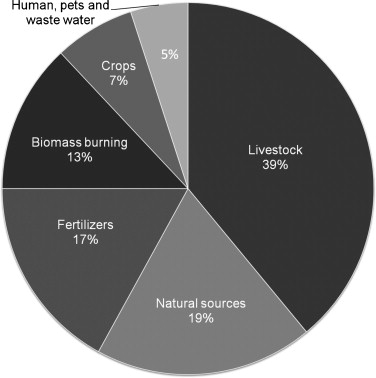
\includegraphics[width=0.5\linewidth]{figures/ammonia-manure} 

}

\caption{Repartition of sources of global ammonia emissions (Galloway et al., 2004).}\label{fig:ammonia-manure}
\end{figure}

Ammonia is emitted from manure in livestock buildings, manure storage
facilities and during manure application to soils. Ammonia in livestock
facilities results primarily from the breakdown of urea (present in
urine) by the enzyme urease (excreted in feces). Typical ammonia levels
in well-ventilated buildings are 10 to 20 ppm. Ammonia can be easily
removed from livestock buildings by proper ventilation because it is
lighter than air.

\begin{table}[t]

\caption{\label{tab:ammonia}Summary of effects in humans following acute ammonia exposure.}
\centering
\begin{tabular}{lll}
\toprule
Concentration (mg/m3) & Exposure time & Effects reported\\
\midrule
3480 & 30 min & Death\\
350 & 30 min & Nasal and throat irritation\\
70 & 6 h & Transient irritation of eyes, nose, and throat\\
56 & 2 h & Coughing, eyes, nose, and throat irritation\\
35 & 2 h & No adverse effect\\
\addlinespace
0.5-37(mean = 3.5) &  & Odour threshold\\
12-14 &  & Odour complaint level\\
\bottomrule
\end{tabular}
\end{table}

\subsubsection{Nitrogen transformations and ammonia production in
manure}\label{nitrogen-transformations-and-ammonia-production-in-manure}

Nitrogen transformations occurring in livestock manure include
mineralization of organic N into NH3, N assimilation into organic
matter, nitrification into nitrite (NO2−) and then into nitrate (NO3−),
and finally denitrification into dinitrogen (N2) with nitrous oxide
(N2O) as a potential by-product (Fig. \ref{fig:ammonia-trans}).

\begin{figure}

{\centering 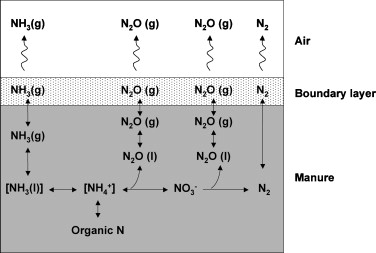
\includegraphics[width=0.5\linewidth]{figures/ammonia-trans} 

}

\caption{Nitrogen (N) transformation in livestock manure and releases to the atmosphere (NH3, ammonia; NH4+, ammonium; NO3−, nitrate; N2O, nitrous oxide; N2, dinitrogen; g, gaseous form; l, liquid form) (adapted from Philippe et al., 2011).}\label{fig:ammonia-trans}
\end{figure}

\subsubsection{Suppression methods}\label{suppression-methods}

\begin{enumerate}
\def\labelenumi{\arabic{enumi}.}
\tightlist
\item
  Decreasing of the length of the time manure remained.
\item
  Keeping buildings and the animals clean and dry.
\item
  Separation manure from urine.
\item
  Using acidifying agents to suppress ammonia emissions from manure.
\item
  Filtration.\\
\item
  Landscaping: Trees, shrubs and other vegetative barriers planted
  around livestock buildings have the potential of reducing ammonia
  emissions.
\end{enumerate}

\subsubsection{Dietary strategies}\label{dietary-strategies}

\begin{enumerate}
\def\labelenumi{\arabic{enumi}.}
\tightlist
\item
  Reduced crude protein (CP) diets containing synthetic amino acids have
  been shown to reduce N excretion, which leads to reduce NH3 emissions.
\item
  Reducing NH3 emissions from the slurry can also be achieved by the
  addition of fibrous feedstuffs in the diet.
\item
  Feed additives: Non-starch polysaccharides enzymes, yucca extract,
  zeolites, probiotics, and so on.
\end{enumerate}

\subsection{Hydrogen sulphide}\label{hydrogen-sulphide}

Hydrogen sulfide (H2S) is a toxic gas and has potential to cause health
problems if the concentration becomes too high. Hydrogen sulphide is
heavier than air, soluble in water, and can accumulate in the livestock
buildings. It has a rotten-egg odour and it can be easily detected at
low concentrations.

\subsubsection{Suppression methods}\label{suppression-methods-1}

\begin{itemize}
\tightlist
\item
  Modifying diets to balance rations reduce hydrogen sulphide emissions.
\item
  Frequent removal of manure from static pits significantly reduces
  hydrogen sulphide.
\item
  Physical, chemical and biological treatment of stored manure such as
  manure additives and oil sprinkling.
\item
  Biofiltration is an effective method for reducing the emissions of
  hydrogen sulphide.
\end{itemize}

\subsection{Particulate matters (Dust)}\label{particulate-matters-dust}

Particulate Matter (PM) is an unusual air pollutant in that it is
defined by its physical morphology rather than chemical identity. The
most common classifications are PM10 (coarse PM), which includes
particles smaller than 10 μm in aerodynamic diameter, and PM2.5 (fine or
respirable PM), which includes particles smaller than 2.5 μm in
diameter.

\begin{itemize}
\tightlist
\item
  \textbf{PM10}: inhalable particles, with diameters that are generally
  10 micrometers and smaller
\item
  \textbf{PM2.5}: fine inhalable particles, with diameters that are
  generally 2.5 micrometers and smaller.
\end{itemize}

\begin{figure}

{\centering 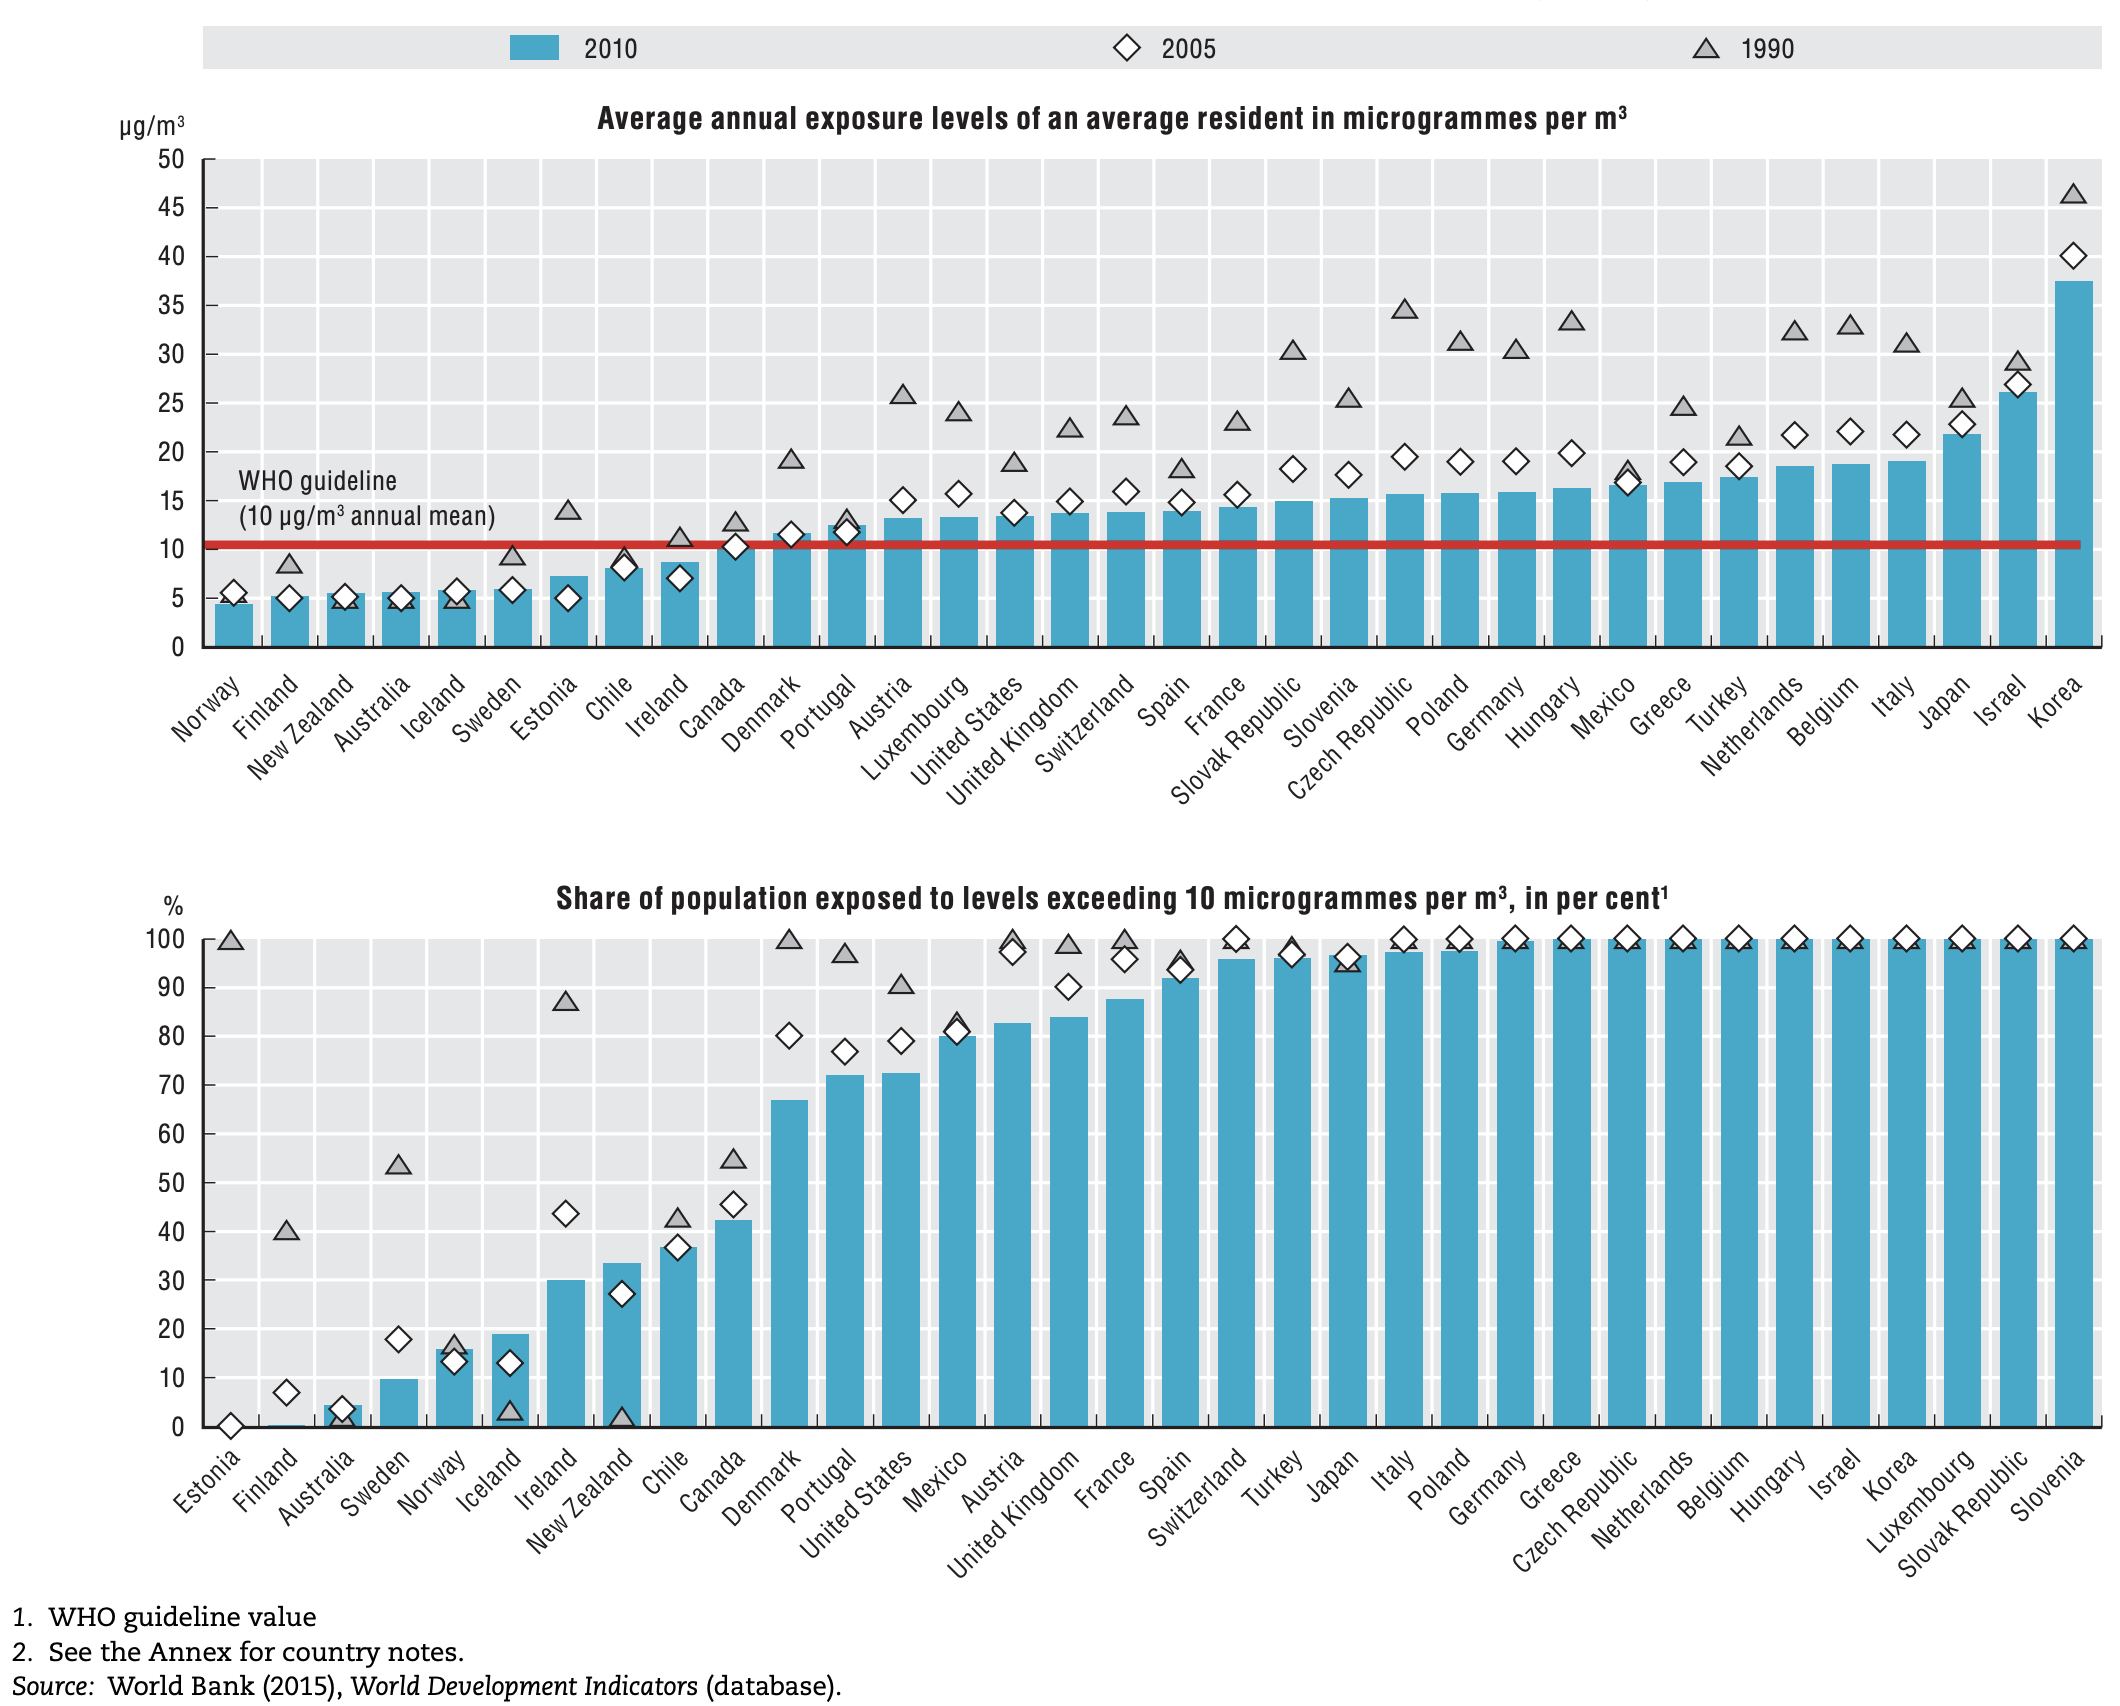
\includegraphics[width=1\linewidth]{figures/pm-oecd} 

}

\caption{Population exposure to fine particulates (PM2.5).}\label{fig:pm-oecd}
\end{figure}

\textbf{Dust from swine/pourtly barns originates from feed, bedding
material, manure and the animals themselves.} Many of the respirable
dust particles are odorous because of their fecal origin. The factors
determining the amount of dust in confinement includes animal activity,
temperature, relative humidity, and ventilation rate, stocking density
and feeding methods.

Dust is related to the odor. Removal of dust in animal production
facilities can reduce the odour in the air by 65-75\% (Hammond and Smith
1981; Hartung 1985.Hartung, 1986; Hoff et al., 1997). Filtering the dust
from the exhaust air reduced VOC--odor emissions from swine buildings by
up to 65\%.

\subsubsection{Factors affecting dust
emissions}\label{factors-affecting-dust-emissions}

\begin{enumerate}
\def\labelenumi{\arabic{enumi}.}
\tightlist
\item
  \textbf{Temperature}: There is the negative correlation between
  outside temperature and the dust concentration.
\item
  \textbf{Relative humidity}: The humid air also increases the moister
  content of the dry manure or and settle dust, so that less dust become
  airborne.
\item
  \textbf{Animal Activity}
\end{enumerate}

\subsubsection{Suppression methods}\label{suppression-methods-2}

\begin{enumerate}
\def\labelenumi{\arabic{enumi}.}
\tightlist
\item
  \textbf{Ventilation}: The major method of controlling dust and air
  contamination in enclosed livestock facilities is by mechanical
  ventilation.
\item
  \textbf{Air Misting}: The oil/water spraying is a promising technique
  for dust control in livestock buildings.
\item
  \textbf{Fibrous Filter}
\item
  \textbf{Wet Collectors}: Wet scrubber using water to capture dust
  particle are very efficient in removing dust particles from air,
  however its use is not recommended in livestock building due to the
  needs for handling large amount of air in livestock buildings.
\end{enumerate}

\chapter{Water quality}\label{water-quality}

\chapter{Cycles of materials}\label{cycles-of-materials}

\section{Ecosystem}\label{ecosystem}

\section{Trophic level}\label{trophic-level}

\section{Carbon cycle}\label{carbon-cycle}

\section{Nitrogen cycle}\label{nitrogen-cycle}

\section{Calcium and Phosphorus
cycle}\label{calcium-and-phosphorus-cycle}

\chapter{Feed ingredients}\label{feed-ingredients}

\section{Agro by-product}\label{agro-by-product}

\chapter{Manure}\label{manure}

\section{Charateristics of animal
manure}\label{charateristics-of-animal-manure}

\section{Manure treatment}\label{manure-treatment}

\subsection{Solid fertilizer
(Composting)}\label{solid-fertilizer-composting}

\subsection{Liquid fertilizer}\label{liquid-fertilizer}

\subsection{Purification}\label{purification}

\subsection{Energy generation}\label{energy-generation}

\subsection{Animal feed}\label{animal-feed}

\chapter{Greenhouse gases}\label{greenhouse-gases}

\chapter{Animal welfare}\label{animal-welfare}

\chapter{ICT technology}\label{ict-technology}

\chapter{Sustainable livestock
industry}\label{sustainable-livestock-industry}

\begin{quote}
``In essence, the conflict between livestock and the environment is a
conflict between different human needs and expectations.'' --- Henning
Steinfeld (FAO)
\end{quote}

\bibliography{book.bib,packages.bib}


\end{document}
